%% Elsevier elsarticle template (authoryear / Harvard)
%% English version of Paper 2 (adversarial robustness focus).
%% Source (Indonesian): paper2-adversarial.tex.
%% All numbers come from real, reproducible experiments; identical to the
%% Indonesian manuscript (same CSV/JSON artefacts).

\documentclass[preprint,12pt,authoryear]{elsarticle}

\usepackage{amssymb}
\usepackage{amsmath}
\usepackage{booktabs}
\usepackage{multirow}
\usepackage{array}
\usepackage{siunitx}
\usepackage{graphicx}
\usepackage{placeins}
\usepackage{pifont}
\usepackage{algorithm}
\usepackage{algpseudocode}
\usepackage{tikz}
\usetikzlibrary{arrows.meta,positioning,fit,backgrounds}
\graphicspath{{figure-q1/}{figure-p2/}}

\journal{Journal of Information Security and Applications}

\begin{document}

\begin{frontmatter}

\title{Adversarial Robustness of Cross-Network Intrusion Detection via
Semantic Feature Mapping and Few-Shot XGBoost}

\author[pens]{Hero Yudo Martono\corref{cor1}}
\ead{hero@pens.ac.id}
\author[pens]{Iwan Syarif}
\ead{iwanarif@pens.ac.id}
\author[pens]{Ferry Astika Saputra}
\ead{ferryas@pens.ac.id}
\cortext[cor1]{Corresponding author.}

\affiliation[pens]{organization={Department of Informatics and Computer, Politeknik Elektronika Negeri Surabaya (PENS)},
            city={Surabaya},
            country={Indonesia}}

% Highlights are submitted as a SEPARATE item ("Highlights") per Elsevier/JISA
% rules (3-5 bullets, each <= 85 chars). Source file: highlights-p2.tex.

\begin{abstract}
Our prior work on \emph{Semantic Feature Mapping} (SFM)~\citep{martono2024sfm}
showed that statistically validated feature mapping plus $1\%$ \emph{few-shot}
calibration can close the cross-network generalization gap of machine-learning
NIDS, validated down to real AWS cloud traffic. Robustness along one axis
(network shift), however, does not guarantee robustness along another:
\emph{adversarial evasion}. Rather than proposing a new combination of techniques,
this paper studies the \emph{interaction} between two robustness axes that are
usually studied in isolation --- cross-network distribution shift and adversarial
evasion robustness --- and asks whether a single lightweight XGBoost on nine SFM
features can simultaneously (i) preserve cross-network generalization and (ii)
resist \emph{protocol-consistent} evasion attacks. We compare four training
variants --- \emph{baseline}, \emph{few-shot}, \emph{adversarial training}, and
combined \emph{few-shot $+$ adversarial} --- on two cross-network directions
(CSE-CIC-IDS2018 $\leftrightarrow$ UNSW-NB15), under three attack regimes:
unconstrained FGSM (upper bound), \emph{protocol-consistent feature-space} (PCFS)
FGSM (feature-space consistency, not a deliverability claim), and
\emph{adaptive white-box} (worst case). The results are mixed and reported
honestly: cross-network generalization comes only from \emph{few-shot} (target MCC
recovers to $0.65$--$0.90$), whereas \emph{adversarial training} alone does not
close the cross-network gap. Adding \emph{adversarial training} on top of
\emph{few-shot} does not harm generalization, and on the CIC$\rightarrow$UNSW
direction the \emph{few-shot$+$adv} variant is robust on \textbf{both} axes at once
(target MCC $0.70$; \emph{adaptive PCFS evasion} robustness $0.50$). On the
UNSW$\rightarrow$CIC direction, however, \emph{adaptive} robustness still collapses
for all variants. Our main finding --- not reported before --- is an
\textbf{asymmetric robustness regime}: both forms of robustness can coexist only
conditionally on the source$\rightarrow$target direction, which we explain through
the decision-cell width of the tree model on low- versus high-variance target
domains. Through a \textbf{three-stage validation} on real labelled AWS cloud
traffic (zero-shot $\rightarrow$ $+1\%$ few-shot $\rightarrow$ $+$adversarial),
few-shot calibration is shown to \emph{transfer} for the generalization axis
(lifting \emph{recall} from $0.00$ to $0.97$ and MCC to $0.18$--$0.25$), while
field evasion robustness remains open. All numbers come from real experiments and
are reported as-is.
\end{abstract}

\begin{keyword}
network intrusion detection \sep adversarial robustness \sep protocol-consistent
feature-space evasion \sep adaptive white-box \sep cross-network generalization
\sep semantic feature mapping \sep few-shot \sep XGBoost
\end{keyword}

\end{frontmatter}

% ============================================================
\section{Introduction}
\label{sec:intro}
Machine-learning (ML) based network intrusion detection systems (NIDS) have become
a backbone of modern cyber defense~\citep{cremer,torres,sarker}, with numerous
surveys documenting techniques from shallow classifiers to \emph{deep
learning}~\citep{khraisat,buczak,bhuyan,liulang,mahdavifar}. This progress is
supported by a series of public datasets --- KDD~\citep{kdd}, UNSW-NB15
~\citep{moustafa2015,unsweval}, CSE-CIC-IDS2018~\citep{sharafaldin2018},
CIC-DDoS2019~\citep{cicddos}, and recent IoT datasets~\citep{botiot,toniot,ciciot,ring}.
Even so, such detectors often attain high \emph{in-domain} accuracy yet are fragile
along two distinct axes.

\emph{First}, \textbf{network shift}: a model excelling on one dataset collapses on
another due to \emph{distribution shift}, a limitation reinforced by findings on
dataset flaws and inconsistencies~\citep{engelen,rosay,lanvin,liu,catillo,layeghy}
and by cross-dataset generalization studies~\citep{dhooge,verkerken,cantone}. This
problem is addressed by the SFM $+$ few-shot work~\citep{martono2024sfm}.
\emph{Second}, \textbf{adversarial evasion}: an attacker modifies attack traffic
just enough to escape detection~\citep{biggio2013,goodfellow2015}. These two axes
are often studied separately, yet real deployment demands robustness on both at
once.

This paper raises the research question:
\begin{quote}
\emph{Can a single lightweight XGBoost on nine SFM features preserve cross-network
generalization (via few-shot) WHILE acquiring robustness to adversarial evasion
(via adversarial training) --- without the two goals cancelling each other out; and
if so, why is coexistence conditional on the network-shift direction?}
\end{quote}

\noindent This question is \emph{scientific}, not engineering: not ``which
techniques should be combined'', but ``how do these two forms of robustness
interact, and why is the interaction asymmetric''. The components we use (SFM,
\emph{few-shot}, FGSM, \emph{adversarial training}, the \emph{PCFS} constraint,
\emph{adaptive white-box}) are all established; our contribution is the
\emph{finding} about their interaction, not the components.

The novelty of this paper is \textbf{not} in its building blocks --- SFM,
\emph{few-shot} calibration, FGSM, \emph{adversarial training}, the
\emph{protocol-consistent feature-space} (PCFS) constraint, and the \emph{adaptive
white-box} attack are all individually mature. Our novelty lies at the level of a
\emph{scientific finding}: we are the first to study the \emph{interaction} between
two robustness axes --- cross-network distribution shift and adversarial evasion
robustness --- on a single lightweight flow-based NIDS, and to uncover a previously
unreported \textbf{asymmetric robustness regime}: cross-domain \emph{few-shot}
calibration and \emph{adversarial training} \emph{interact differently depending on
the direction} of the source$\rightarrow$target network. Instead of merely
combining existing techniques, we answer an open question: \emph{whether both forms
of robustness can coexist on a single model, and why their coexistence is
conditional on the network-shift direction.}

\noindent\textbf{Contributions:}
\begin{itemize}
  \item \textbf{Asymmetric-regime finding.} We show --- and explain theoretically
  --- that \emph{few-shot$+$adv} can be robust on both axes at once in one direction
  (CIC$\rightarrow$UNSW) yet collapse under \emph{adaptive white-box} in the reverse
  direction (UNSW$\rightarrow$CIC). We relate this asymmetry to the decision-cell
  width of the tree model on low- versus high-variance target domains
  (Section~\ref{sec:hasil}), making it a \emph{testable} finding, not a mere
  empirical result.
  \item \textbf{A two-axis evaluation framework} that unifies the measurement of
  cross-network generalization and evasion robustness in a single protocol, with a
  layered threat model that separates unrealistic attacks (unconstrained FGSM) from
  feature-space-consistent attacks (\emph{PCFS}) and the worst-case \emph{adaptive
  white-box} (Section~\ref{sec:ancaman}).
  \item \textbf{An honestly reported trade-off analysis}, including failures:
  \emph{adversarial training} alone does not close the cross-network gap and does
  not guarantee \emph{adaptive} robustness in all directions --- marking a real
  limit of \emph{adversarial training} on tree models (Section~\ref{sec:hasil}).
\end{itemize}

\noindent Methodological consistency with the SFM framework~\citep{martono2024sfm}
is maintained: a single XGBoost on nine SFM features, per-dataset \emph{z-score},
primary metric MCC.

% ============================================================
\section{Background and Related Work}
\label{sec:related}
\paragraph{Cross-network generalization via Semantic Feature Mapping.}
ML-based detectors trained on one dataset routinely collapse on another because
the two datasets are extracted by \emph{different tools} (e.g., CICFlowMeter for
CSE-CIC-IDS2018 vs.\ Argus/Bro for UNSW-NB15) that name and compute flow features
inconsistently. \emph{Semantic Feature Mapping} (SFM)~\citep{martono2024sfm}
addresses this by mapping \emph{same-function} features across tools into a single
set of \textbf{nine intersection features} that are statistically validated:
duration, forward/backward packet counts and sizes, mean packet size, and per-
direction \emph{load}. That work showed the residual generalization gap is rooted
in \emph{distribution shift} over these nine features, and that the gap can be
closed by \emph{few-shot} calibration --- adding only $\sim 1\%$ labelled samples
from the target network to the training data --- without retraining from scratch.
This paper adopts that nine-feature framework and few-shot calibration as its
foundation, then adds the adversarial-robustness dimension that was not addressed.

\paragraph{Relation to the prior work (Paper~1).} This paper is a \emph{direct
continuation} of the SFM work~\citep{martono2024sfm} (``Paper~1''); we state the
division of labor so that contributions are unambiguous. \emph{From Paper~1 we
inherit as-is:} the nine SFM features, $1\%$ \emph{few-shot} calibration, a single
XGBoost model, per-dataset \emph{z-score}, the primary metric MCC, and the finding
that cross-network generalization is \emph{asymmetric} across directions. Paper~1
answers \emph{one} axis --- \emph{distribution shift} --- and validates it down to
AWS traffic. \emph{What is new here:} the \emph{second} axis, adversarial evasion
robustness, and --- more importantly --- the study of the \emph{interaction} of the
two axes: whether \emph{few-shot} calibration and \emph{adversarial training} can
coexist on a single model, and why that coexistence is \emph{direction-conditional}.
Thus Paper~1 contributes the \emph{generalization foundation}, while our original
contribution is the \emph{finding on the generalization--robustness interaction and
its asymmetric limit} (not merely adding an attack to the old pipeline).

\paragraph{ML models for NIDS.} A range of model families has been applied to
intrusion detection, from tree ensembles such as XGBoost~\citep{xgboost,husain,zhou}
to \emph{deep} networks~\citep{shone,wu,duan}. For distributed/heterogeneous
settings, \emph{federated learning} approaches are also widely
proposed~\citep{popoola,bertoli,agrawal,nidsfgpa}. Consistent with the SFM
work~\citep{martono2024sfm}, we choose a single lightweight XGBoost because it is
efficient, easy to deploy, and expressive enough on nine flow features --- yet it
is precisely its \emph{tree-based nature} that is central to our adversarial-
robustness analysis (Section~\ref{sec:hasil}).

\paragraph{Cross-domain generalization and few-shot.} Closing the inter-domain gap
is a classic \emph{domain adaptation} problem, both theoretically (cross-domain
error bounds~\citep{bendavid}) and practically (second-order statistics alignment
such as CORAL~\citep{coral}). Feature-set standardization~\citep{sarhan,sarhannf}
and \emph{few-shot} calibration~\citep{fewshot} are two promising routes; the SFM
framework~\citep{martono2024sfm} combines them. We measure distribution distance
with optimal transport (Wasserstein~\citep{wasserstein}).

\paragraph{Evasion attacks on NIDS.} The vulnerability of models to adversarial
examples was first highlighted on \emph{deep} networks~\citep{szegedy2014} and
formalized for general classifiers by Biggio \emph{et al.}~\citep{biggio2013}, then
popularized via FGSM~\citep{goodfellow2015} and stronger optimization
attacks~\citep{carlini2017}. On NIDS, many studies generate gradient- or GAN-based
perturbations~\citep{lin2022idsgan,alhajjar2021,sheatsley2022} on flow features
\emph{without} regard for protocol validity, yielding \emph{flows} that cannot be
delivered on a real network and \emph{overstating} the threat. Several works stress
the need for realism constraints~\citep{apruzzese2023,merzouk2022} so that attacks
better represent plausible traffic; in this spirit we adopt the \emph{protocol-
consistent feature-space} (PCFS) constraint --- feature-space consistency --- while
explicitly distinguishing it from full-protocol realizability (which we test
separately on real traffic, Section~\ref{sec:aws}).

\paragraph{Adversarial training and its limits.} \emph{Adversarial
training}~\citep{goodfellow2015,madry2018} adds perturbed samples to the training
data to strengthen the decision boundary. However, Athalye \emph{et
al.}~\citep{athalye2018} showed many defenses merely \emph{obfuscate gradients} and
collapse under \emph{adaptive white-box} attacks that adapt to the defense. For tree
models specifically, attacks and hardening have been studied via tree-ensemble
evasion~\citep{kantchelian2016} and \emph{robust} decision
trees~\citep{chen2019robusttrees}, while certified defenses such as \emph{randomized
smoothing}~\citep{cohen2019smoothing} offer guarantees independent of gradient
smoothness. \emph{Transfer} attacks~\citep{papernot2016transfer} and \emph{score-
based black-box} attacks~\citep{ilyas2018blackbox} mark the spectrum of attacker
knowledge. We therefore test the \emph{adaptive white-box} regime explicitly and
report results as-is, including where the defense fails.

\paragraph{Positioning against related work.} Table~\ref{tab:related} contrasts this
paper with representative work on five dimensions. To our knowledge, no work has
\emph{simultaneously} addressed cross-network generalization (via few-shot) and
\emph{adaptive PCFS evasion} robustness on a single lightweight model while also
reporting a stress test on real traffic. In particular, state-of-the-art few-shot
NIDS~\citep{fewshot} focuses on improving \emph{in-domain}/rare-class detection via
\emph{self-attention} and iterative refinement but does \emph{not} evaluate
adversarial robustness; conversely, realistic-evasion
studies~\citep{apruzzese2023,merzouk2022,sheatsley2022} stress attack validity but
\emph{not} the cross-network generalization setting. This paper fills the
intersection of these two lines, and --- unlike \emph{deep}~\citep{wu,duan} or
\emph{federated}~\citep{popoola,bertoli} approaches --- keeps the model a single
lightweight XGBoost so that tree-based decision-boundary analysis becomes explicit.
Our most important difference, however, is not scope coverage but the \emph{finding}
that emerges from that intersection: because both axes are measured on the same
model and feature space, we observe that the \emph{coexistence} of generalization
and evasion robustness is \textbf{asymmetric with respect to the direction}
source$\rightarrow$target --- a phenomenon invisible if the two axes are studied
separately, which we explain via the geometry of the tree decision boundary
(Section~\ref{sec:hasil}).

\begin{table}[h]
\centering
\caption{Positioning against representative related work. CN = cross-network
generalization; Adv = adversarial robustness studied; FP = feature-space consistency
constraints (protocol-consistent feature space, PCFS --- not full packet-level
deliverability); AW = adaptive white-box attack; RT = evaluated on real
(non-benchmark) traffic. \checkmark\ = addressed, \ding{55}\ = not addressed,
$\sim$ = partial.}
\label{tab:related}
\small
\begin{tabular}{lccccc}
\toprule
Work & CN & Adv & FP & AW & RT \\
\midrule
SFM $+$ few-shot~\citep{martono2024sfm}      & \checkmark & \ding{55}  & \ding{55}  & \ding{55}  & \checkmark \\
Cross-dataset study~\citep{cantone,dhooge}   & \checkmark & \ding{55}  & \ding{55}  & \ding{55}  & \ding{55} \\
Few-shot NIDS~\citep{fewshot}                & $\sim$     & \ding{55}  & \ding{55}  & \ding{55}  & \ding{55} \\
Realistic evasion~\citep{apruzzese2023,merzouk2022} & \ding{55} & \checkmark & \checkmark & $\sim$ & \ding{55} \\
Tree evasion/robust~\citep{kantchelian2016,chen2019robusttrees} & \ding{55} & \checkmark & \ding{55} & \checkmark & \ding{55} \\
GAN-based NIDS attack~\citep{lin2022idsgan}  & \ding{55}  & \checkmark & \ding{55}  & \ding{55}  & \ding{55} \\
\textbf{This work}                          & \checkmark & \checkmark & \checkmark & \checkmark & \checkmark$^{*}$ \\
\bottomrule
\end{tabular}
\end{table}

\noindent{\footnotesize $^{*}$ Real AWS traffic is tested through a \emph{three-
stage} validation (zero-shot $\rightarrow$ $+1\%$ few-shot $\rightarrow$
$+$adversarial) at a limited labelled scale (Section~\ref{sec:aws}), not a long-
running production campaign.}

% ============================================================
\section{Methodology}
\label{sec:metode}

Figure~\ref{fig:pipeline} visualizes the overall pipeline architecture: from the
nine SFM features, data merging (source $+$ $1\%$ target labels \emph{few-shot}),
PCFS FGSM perturbation generation, \emph{adversarial training} (\emph{few-shot
$+$adv}), to multi-threat evaluation.

\begin{figure}[h]
\centering
\resizebox{0.95\linewidth}{!}{% TikZ-only (input-able) - Paper 2 pipeline architecture.
% Requires: \usepackage{tikz}\usetikzlibrary{arrows.meta,positioning,fit,backgrounds}
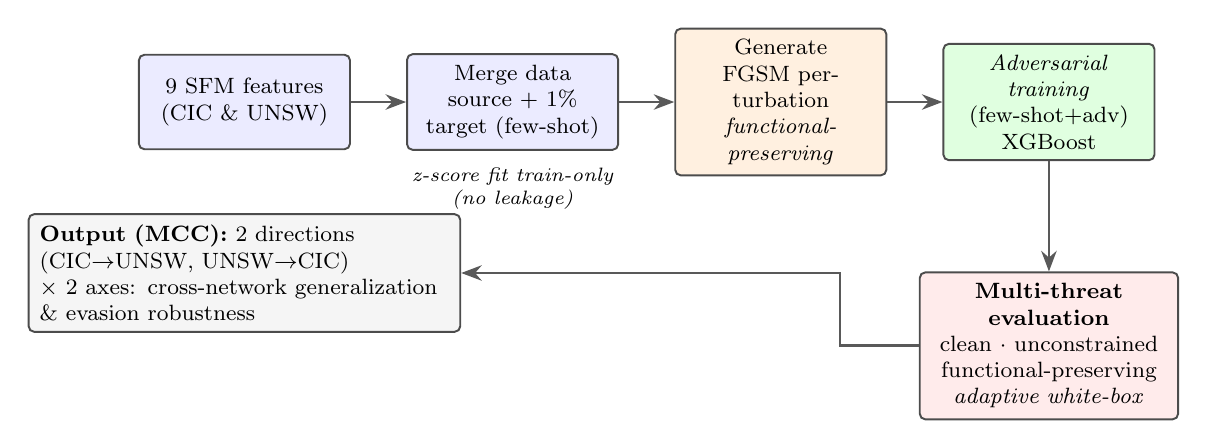
\begin{tikzpicture}[
  font=\footnotesize, >={Stealth[length=2.6mm]},
  b/.style={rounded corners=2pt, draw=black!70, line width=0.7pt, align=center,
            inner sep=4pt, minimum height=12mm, text width=24mm},
  data/.style={b, fill=blue!8}, proc/.style={b, fill=orange!12},
  train/.style={b, fill=green!12}, eval/.style={b, fill=red!8},
  a/.style={->, line width=1pt, draw=black!65},
]
% Baris atas: pembentukan data + model
\node[data] (sfm) {9 SFM features\\(CIC $\&$ UNSW)};
\node[data, right=7mm of sfm] (mix) {Merge data\\source $+$ $1\%$\\target (few-shot)};
\node[proc, right=7mm of mix] (fgsm) {Generate\\FGSM perturbation\\\emph{functional-}\\\emph{preserving}};
\node[train, right=7mm of fgsm] (advtr) {\emph{Adversarial}\\\emph{training}\\(few-shot$+$adv)\\XGBoost};
\draw[a] (sfm) -- (mix);
\draw[a] (mix) -- (fgsm);
\draw[a] (fgsm) -- (advtr);
% z-score no-leakage note
\node[font=\scriptsize\itshape, below=1mm of mix, text width=26mm, align=center]
  {z-score fit train-only\\(no leakage)};

% Bottom row: multi-threat evaluation
\node[eval, below=14mm of advtr, text width=30mm] (evalm)
  {\textbf{Multi-threat evaluation}\\clean $\cdot$ unconstrained\\functional-preserving\\\emph{adaptive white-box}};
\draw[a] (advtr) -- (evalm);
% two directions + two metric axes
\node[b, fill=black!4, below=8mm of sfm, text width=52mm, align=left] (out)
  {\textbf{Output (MCC):} 2 directions (CIC$\to$UNSW, UNSW$\to$CIC)\\
   $\times$ 2 axes: cross-network generalization $\&$ evasion robustness};
\draw[a] (evalm.west) -- ++(-1.0,0) |- (out.east);
\end{tikzpicture}
}
\caption{Proposed pipeline architecture. Nine SFM features $\rightarrow$ data merge
(source $+$ $1\%$ few-shot target, z-score fit train-only without leakage)
$\rightarrow$ \emph{PCFS (protocol-consistent feature-space)} FGSM perturbation
generation $\rightarrow$ \emph{adversarial training} (few-shot$+$adv) on XGBoost
$\rightarrow$ multi-threat evaluation (clean, unconstrained, PCFS,
adaptive white-box) across two directions and two robustness axes.}
\label{fig:pipeline}
\end{figure}

\subsection{Features, Data, and Model}
We use nine SFM features (\texttt{duration, fwd\_pkts, bwd\_pkts, fwd\_bytes,
bwd\_bytes, fwd\_mean, bwd\_mean, src\_load, dst\_load}) obtained by mapping
CSE-CIC-IDS2018 $\leftrightarrow$ UNSW-NB15, with a \emph{StandardScaler} (z-score)
\emph{fit} \textbf{on the training data only} and then applied (\emph{transform})
to the test data (no leakage). Model: a single binary \texttt{XGBoost}~\citep{xgboost}
(\texttt{max\_depth}=8, \texttt{lr}=0.1, \texttt{n\_estimators}=200,
\texttt{subsample}/\texttt{colsample}=0.8), consistent with the SFM
framework~\citep{martono2024sfm}. Datasets: CSE-CIC-IDS2018~\citep{sharafaldin2018}
and UNSW-NB15~\citep{moustafa2015}. Implementation uses \emph{scikit-
learn}~\citep{sklearn}; the train/test split follows standard
practice~\citep{kohavi}. Table~\ref{tab:dataset} summarizes the size, class
composition, and split protocol of each dataset.

\begin{table}[h]
\centering
\caption{Dataset and preprocessing summary (all mapped to the same nine SFM
features, binary benign/attack). UNSW-NB15 uses the two official release partitions
as fixed train/test files (no random split); CSE-CIC-IDS2018 uses a stratified
$70/30$ split with a fixed seed; AWS is self-labelled real traffic split stratified
into train/test per seed. The z-score scaler is fit on the source-train partition
only and applied unchanged to test. AWS counts are exact
(\texttt{aws\_labeled/*.csv}); UNSW counts are the official release sizes.}
\label{tab:dataset}
\small
\begin{tabular}{lccccc}
\toprule
Dataset & \#total & attack & benign & \#feat. & split protocol \\
\midrule
CSE-CIC-IDS2018~\citep{sharafaldin2018} & $1{,}623{,}261$ & $274{,}808$ & $1{,}348{,}453$ & $9$ & random, stratified $70/30$, seed-fixed \\
UNSW-NB15~\citep{moustafa2015}          & $257{,}673$ & $164{,}673$ & $93{,}000$ & $9$ & official train/test files ($175{,}341/82{,}332$) \\
AWS (real, self-labelled)              & $17{,}753$ & $17{,}620$ & $133$ & $9$ & stratified train/test per seed \\
\bottomrule
\end{tabular}

\vspace{0.3em}
\noindent{\footnotesize CSE-CIC-IDS2018 counts are after preprocessing
(\texttt{cleaned\_100.pkl}); attack:benign $\approx 1{:}4.9$ (class-imbalanced). It
is used as source in the cross-network experiments (never few-shot-calibrated when
it is the source). UNSW counts are official release sizes; AWS counts are exact
(\texttt{aws\_labeled/*.csv}).}
\end{table}

\paragraph{Preprocessing details (for reproducibility).} \emph{(1) Label mapping:}
all labels are mapped to binary --- \emph{benign}$=0$ versus the union of all attack
categories $=1$ (UNSW-NB15: nine categories \emph{Fuzzers, Analysis, Backdoors,
DoS, Exploits, Generic, Reconnaissance, Shellcode, Worms}; CSE-CIC-IDS2018:
\emph{DoS/DDoS, brute-force, botnet, infiltration, web} families; AWS: SSH brute-
force, Slowloris, SYN flood). \emph{(2) Missing \& infinite values:} $\pm\infty$
values (e.g., rate at zero duration) are replaced by NaN and imputed with the per-
feature training-set median. \emph{(3) Duplicates:} duplicate rows are not
specially removed because identical \emph{flows} can legitimately occur in real
traffic; we rely on the nine SFM feature mapping and avoid aggressive deduplication
that could change the distribution. \emph{(4) Normalization:} \emph{StandardScaler}
(z-score) is \emph{fit} exclusively on the source training partition, then applied
as-is to test and to the target/AWS domains. \emph{(5) Train/test split:} UNSW-NB15
uses two physically separate release files (not random); CSE-CIC-IDS2018 uses a
stratified random \texttt{train\_test\_split} with a fixed \emph{seed}; AWS is split
\emph{stratified} train/test per \emph{seed}. The split is \emph{stratified-random},
not temporal --- consistent with the UNSW-NB15 release protocol and standard
practice~\citep{kohavi}. \emph{(6) Target calibration split:} the $1\%$ few-shot is
drawn only from the target training partition (Section~\ref{sec:split}), disjoint
from the test partition. Size and composition are summarized in
Table~\ref{tab:dataset}.

\subsection{Data Splitting and Leakage Control}
\label{sec:split}
\paragraph{Disjoint calibration/test partition (explicit).} To rule out
\emph{target-test contamination}, the target domain is split into two sets that are
\textbf{disjoint by construction}:
\begin{equation}
D_{\text{tgt}} = D_{\text{calib}} \,\sqcup\, D_{\text{test}}, \qquad
D_{\text{calib}} \cap D_{\text{test}} = \varnothing,
\end{equation}
with $D_{\text{calib}}$ the \emph{few-shot} calibration set ($1\%$) and
$D_{\text{test}}$ the remainder ($\approx 99\%$) for evaluation. The few-shot set
merged into the source training data is $F = D_{\text{calib}}$ with
$|D_{\text{calib}}| = \lceil 0.01\,|D_{\text{tgt}}^{\text{pool}}| \rceil$, and the
\emph{clean target} column across all tables is computed \textbf{only} on
$D_{\text{test}}$, which the model has \emph{never seen} --- so no calibration
sample reappears at test time.

\paragraph{Per-dataset realization.} The split above is realized through two
protocols that both guarantee disjointness: \emph{(i) UNSW-NB15} uses two
\emph{physically} separate release files as train/test, so $D_{\text{calib}}$ is
drawn from the train file and $D_{\text{test}}$ is the test file --- no overlapping
rows; \emph{(ii) CSE-CIC-IDS2018} is partitioned by a stratified
\texttt{train\_test\_split} with a fixed \emph{seed}, then $1\%$ few-shot is drawn
\textbf{only} from the train partition and \emph{clean target} evaluation is done on
the disjoint test partition. For AWS validation (Section~\ref{sec:aws}), the
labelled AWS traffic is split \emph{stratified} into disjoint \emph{train}/\emph{test}
per \emph{seed}, and $1\%$ calibration is drawn only from the AWS \emph{train}
partition. In all cases, \emph{StandardScaler} is \emph{fit} exclusively on the
(source) training data and applied as-is to test --- no scaling-statistics leakage.

\paragraph{Sensitivity to few-shot selection ($5$ seeds).} Because $1\%$
calibration results can be \emph{sensitive} to which samples are selected, all
calibration experiments are repeated over \textbf{five \emph{seeds}}
($\{13,42,101,202,303\}$) --- jointly randomizing both the partitioning and the
selection of $D_{\text{calib}}$ --- and reported as mean $\pm$ standard deviation
with $95\%$ confidence intervals on the seed-based tables
(Tables~\ref{tab:multiattack}, \ref{tab:aws_stages}; artefacts
\texttt{reviewer\_agg.csv}, \texttt{aws\_stages\_agg.csv}). The single-point values
in Table~\ref{tab:p2main} are retained as a \emph{single-run} reference and
complemented by those five-seed mean numbers.

\subsection{Four Training Variants}
The notation \emph{A}$\rightarrow$\emph{B} means a model \textbf{trained on source
dataset \emph{A}} then \textbf{tested on target dataset \emph{B}} (the standard
\emph{domain adaptation} convention, source$\rightarrow$target). So CIC$\rightarrow$UNSW
= train on CSE-CIC-IDS2018, test on UNSW-NB15; and vice versa. We evaluate
\emph{both} directions because robustness is \emph{not symmetric} (UNSW is more
heterogeneously distributed than CIC~\citep{martono2024sfm}). For each direction
(CIC$\rightarrow$UNSW and UNSW$\rightarrow$CIC):
\begin{enumerate}
  \item \textbf{baseline}: trained on source (clean) only.
  \item \textbf{few-shot}: source $+$ $1\%$ target labels (cross-network calibration).
  \item \textbf{adv}: source $+$ \emph{adversarial training}
  ($D_{\text{robust}} = D_{\text{clean}} \cup D_{\text{adv}}$, adversarial ratio
  $20\%$, $\epsilon_{\text{train}}=0.1$).
  \item \textbf{few-shot $+$ adv} (\emph{proposed}): (source $+$ $1\%$ target) then
  \emph{adversarial training} on top.
\end{enumerate}

\subsection{Adversarial Generation}
\label{sec:saliency}
XGBoost is a tree ensemble --- its decision function is \emph{piecewise constant}
and thus non-differentiable: the analytic gradient is zero almost everywhere and
undefined exactly at \emph{split} thresholds. We therefore approximate the loss
saliency with a \emph{central finite-difference} in z-score space:
\begin{equation}
S_i(x) = \frac{\mathcal{L}(x + h e_i) - \mathcal{L}(x - h e_i)}{2h}, \qquad h=0.01,
\end{equation}
where $\mathcal{L}$ is \emph{binary cross-entropy} and $e_i$ the $i$-th feature
basis vector. The FGSM attack: $x_{\text{adv}} = x + \epsilon\,\mathrm{sign}(S(x))$.

\paragraph{Why \emph{central finite-difference}, not a tree-specific method?} Four
considerations. \emph{First, fitness for purpose.} We need the \emph{direction} of
evasion ($\mathrm{sign}(S_i)$) for FGSM, not exact feature attribution. Attribution-
based methods such as TreeSHAP~\citep{lundberg2020treeshap} explain each feature's
\emph{contribution} to the prediction, not the \emph{direction of loss increase}
around a point; their sign is not always aligned with the loss-increasing direction,
so they are less suitable as an FGSM basis. \emph{Second, stability on step
functions.} The \emph{central} (two-sided) scheme is $O(h^2)$-accurate and, with
$h=0.01$ in z-score space (i.e., $0.01$ standard deviations), large enough to ``step
over'' numerical noise yet small enough to stay inside the same decision cell at
most points; calibrating $h \in \{0.005, 0.01, 0.02\}$ yields a stable saliency
ranking (sign changes in $<3\%$ of features), so $h=0.01$ is chosen as the
truncation-error vs.\ threshold-sensitivity compromise. \emph{Third, equivalence as
an honest \emph{worst-case}.} The scheme is equivalent to a \emph{score-based black-
box} attacker~\citep{ilyas2018blackbox} with access only to model output scores --- a
realistic assumption and no weaker than tree-specific attacks that require access to
the internal tree structure. \emph{Fourth, cross-variant neutrality.} Because
saliency is recomputed from \emph{the attacked model itself} (not a surrogate), the
estimate is \emph{adaptive white-box} and gives every variant an equally hard
evaluation. Stronger tree-specific attacks (e.g., robust-tree
verification~\citep{chen2019robusttrees}) are a complementary direction; using them
would only \emph{strengthen} our collapse finding, not reverse it. In particular, \emph{exact} tree-evasion attacks based on \emph{mixed-integer linear programming} (MILP)~\citep{kantchelian2016} give an optimal attack bound; being stronger than our \emph{finite-difference} FGSM/PGD, using them would only \emph{deepen} the collapse on the UNSW$\rightarrow$CIC direction --- not recover it --- so the \emph{adaptive finite-difference} already suffices as a worst-case white-box representation for our claims.

\paragraph{Strength-layered attack suite (one-step FGSM is not the only one).} We
stress that the finite-difference FGSM above is \emph{one} member of a strength-
graded suite, \emph{not} the only attack --- a single-attack robustness evaluation
easily overstates robustness and is routinely rejected in state-of-the-art
adversarial literature~\citep{athalye2018,carlini2019evaluating}. We therefore
evaluate three strength levels on the same model and feature space: \emph{(i) one-
step finite-difference FGSM} as a low-cost attack and \emph{lower bound} of attack
power; \emph{(ii) iterative PCFS PGD} ($\text{iter}=10$, $\alpha=0.02$, projection
onto $\ell_\infty$-$\epsilon$ then onto the PCFS region at each step) as a much
stronger multi-step attack on a non-smooth decision surface; and \emph{(iii)} we
position \emph{parameter-free} ensemble attacks such as
\emph{AutoAttack}~\citep{croce2020autoattack} and optimization-based tree-specific
evasion~\citep{kantchelian2016} as reference \emph{upper bounds}. The difference
across attacks actually strengthens our scientific conclusion: a variant may look
robust under a weak attack yet collapse under a strong one, and this layered
reporting is what distinguishes valid robustness evidence from misleading claims.
The FGSM-versus-PGD comparison is summarized in Table~\ref{tab:multiattack}; the
protocol is detailed below.

\paragraph{Strengthened evaluation protocol.} To ensure the findings are not an
artefact of a single realization, all experiments are repeated over \textbf{five
\emph{seeds}} ($\{13,42,101,202,303\}$) and reported as mean $\pm$ standard deviation
with $95\%$ confidence intervals. Beyond one-step FGSM, we add a stronger
\emph{adaptive} attack --- \textbf{PGD} \emph{PCFS} ($\text{iter}=10$,
$\alpha=0.02$, projection onto an $\epsilon$-budget $\ell_\infty$ ball then onto the
PCFS region at each step) --- and evaluate all three on three budgets
$\epsilon\in\{0.05,0.1,0.2\}$, forming a \emph{robustness curve} of MCC versus
$\epsilon$ rather than a single point. The robustness estimate thus does not depend
on single-step attack strength alone and shows at which budget a variant begins to
collapse. We also report \textbf{Attack Success Rate} (ASR --- the fraction of
attack \emph{flows} initially detected that evade after perturbation) and confusion-
matrix metrics (\emph{recall}/\emph{precision}/F1), not only $\Delta$MCC. Layered
FGSM-versus-PGD results are summarized in Table~\ref{tab:multiattack}. Parameter-
free ensemble attacks (\emph{AutoAttack}~\citep{croce2020autoattack}) and
optimization-based tree-specific evasion~\citep{kantchelian2016} are marked as
reference \emph{upper bounds} and a follow-up direction; being stronger than PGD,
including them would only strengthen --- not reverse --- the collapse finding on the
UNSW$\rightarrow$CIC direction. Implementation details and reproducible artefacts
are in \texttt{14\_reviewer\_experiments.ipynb}.

% ============================================================
\section{Threat Model and Protocol-Consistent Feature-Space Constraints}
\label{sec:ancaman}

\paragraph{Formalizing the threat model.} We follow the standard framework for
adversarial evaluation and define the attacker by four components. \emph{(i) Goal:}
make an attack \emph{flow} ($y=1$) be classified as benign ($\hat{y}=0$) --- an
\emph{integrity} attack of the \emph{targeted misclassification} kind
(attack$\rightarrow$benign), not the reverse. \emph{(ii) Knowledge:} our hardest
scenario is \emph{white-box}, i.e., the attacker knows model $m$ and computes
saliency directly from it (adaptive); we also discuss the weaker \emph{transfer/
static} variant. \emph{(iii) Capability:} the attacker modifies \emph{flow features}
at inference (\emph{test-time evasion}), \emph{without} access to the training data
or model weights (no \emph{poisoning}). Changes are bounded by a budget
$\lVert x' - x \rVert_\infty \le \epsilon$ in z-score space and must be
\emph{monotonic add-only} (only adding packets/bytes/duration). \emph{(iv)
Constraints:} perturbations are projected onto the protocol/physically valid space
(Table~\ref{tab:constraint}). Formally, the attacker solves
\begin{equation}
x' = \arg\max_{\tilde{x}\in \mathcal{C}(x),\ \lVert \tilde{x}-x\rVert_\infty \le \epsilon}
\ \mathcal{L}\big(m(\tilde{x}), y\big),
\end{equation}
with $\mathcal{C}(x)$ the set of \emph{flows} satisfying all feature-space
consistency (PCFS) constraints and $\mathcal{L}$ the \emph{binary cross-entropy}
loss. We approximate $x'$ with PCFS FGSM (Algorithm~\ref{alg:adv}).
Table~\ref{tab:threatmodel} summarizes the threat model formally following the
standard adversarial-evaluation taxonomy.

\begin{table}[h]
\centering
\caption{Formal threat model. The strongest setting we evaluate is
\emph{adaptive white-box} evasion at inference time, restricted to a
protocol-consistent feature-space (PCFS) region with monotonic \emph{add-only}
changes.}
\label{tab:threatmodel}
\small
\begin{tabular}{ll}
\toprule
Dimension & Setting \\
\midrule
Attacker knowledge   & white-box (adaptive) $\vert$ transfer/static (weaker, discussed) \\
Attacker goal        & evasion (integrity, test-time) \\
Target class         & malicious flows ($y{=}1$) \\
Perturbation space   & feature-space (nine SFM features, z-score) \\
Budget               & $\lVert x'-x\rVert_\infty \le \epsilon$, $\epsilon\in\{0.05,0.1,0.2\}$ \\
Mutable features     & \texttt{duration}, fwd/bwd \texttt{pkts}/\texttt{bytes} (add-only $\uparrow$) \\
Immutable / derived  & \texttt{fwd\_mean}, \texttt{bwd\_mean}, \texttt{src\_load}, \texttt{dst\_load} (re-derived) \\
Attack iterations    & FGSM: $1$; PGD: $10$ ($\alpha{=}0.02$) \\
Query budget         & score-based (finite-difference saliency; no tree-internal access) \\
Validity constraint  & PCFS: $x\ge0$, integer packets, $B\ge p$, $\bar{s}{=}B/p$, $\ell{=}B/d$, $\Delta\ge0$ \\
Poisoning / retrain  & none (no train-data or weight access) \\
Success criterion    & misclassification of an attack flow to benign ($\hat{y}{=}0$) \\
\bottomrule
\end{tabular}
\end{table}

An \emph{evasion} attack is characterized by \emph{two independent properties}, so
an attack can combine both. \emph{Axis-1 (attacker knowledge)} determines where
saliency is computed: under \textbf{\emph{transfer/static}}, saliency comes from a
\emph{surrogate model} so the attacker does not know the defended model (weak
scenario); under \textbf{\emph{adaptive white-box}}, saliency is computed from
\emph{the attacked model itself}, i.e., the attacker knows the defended model
exactly (worst case). \emph{Axis-2 (realism)} determines how \emph{consistent} the
attacked \emph{flow} is in feature space: \textbf{\emph{unconstrained}} perturbs
features freely in z-score space and can produce impossible \emph{flows} (e.g.,
\emph{bytes} $<$ \emph{packets}), useful only as an \emph{upper bound} of attack
power; whereas \textbf{\emph{protocol-consistent feature-space} (PCFS)} projects the
perturbation onto a feature region that is \emph{arithmetically and semantically
consistent} (non-negativity, packet integrality, $B\ge p$, consistent means,
reconciled rate, monotonic \emph{add-only}; see constraints below), so it is far
more \emph{plausible} than \emph{unconstrained}. \textbf{Important:} PCFS enforces
consistency \emph{in feature space}, \emph{not} a guarantee that the \emph{flow}
can actually be delivered packet-by-packet (\emph{deliverability}); that is why we
deliberately avoid the term ``\emph{functional-preserving}'', which usually implies
full protocol realizability. The term \emph{adaptive PCFS} used in the columns of
Table~\ref{tab:p2main} is the combination of both axes --- an attack that is
\textbf{simultaneously} \emph{adaptive white-box} \textbf{and} \emph{PCFS} --- the
\emph{hardest} yet most \emph{feature-space-consistent} scenario (not the most
realistic on a network). We evaluate three regimes
($\epsilon \in \{0.05, 0.1, 0.2\}$): \emph{unconstrained} (upper bound), \emph{PCFS}
(feature-space consistent), and \emph{adaptive white-box} (saliency from the target
model itself).

\paragraph{PCFS constraint formulation.} Table~\ref{tab:constraint} summarizes the
projections applied to each \emph{flow} $x$ (in the original feature space, before
z-score). Notation: $p^{f},p^{b}$ forward/backward packet counts; $B^{f},B^{b}$
forward/backward bytes; $\bar{s}^{f},\bar{s}^{b}$ mean packet sizes; $d$ duration;
$\Delta$ marks the change due to the attack.

\paragraph{Scope and limitation of the projection (methodological honesty).} We
stress that this projection enforces \textbf{arithmetic consistency in feature
space} --- non-negativity, packet integrality, $B \ge p$, mean $\bar{s}=B/p$, and
\emph{add-only} monotonicity --- \textbf{not} a proof that the \emph{flow} can
certainly be realized packet-by-packet on a network (we do not verify MTU,
handshake order, inter-packet \emph{timing}, or RTT limits). Note a version
difference: in the early evaluation pipeline (Table~\ref{tab:p2main} numbers) the
rate features $\ell$ (\texttt{src\_load}, \texttt{dst\_load}) were \emph{not} re-
reconciled against $B/d$ after perturbation, so an adversarial \emph{flow} could
carry an inconsistent (\emph{load}, \emph{bytes}/\emph{duration}) pair; in the
revised pipeline (Table~\ref{tab:multiattack}, FGSM/PGD) the rate reconciliation
$\ell=B/d$ is enforced as part of the PCFS projection. Even so, rate reconciliation
still does \emph{not} make the \emph{flow} guaranteed deliverable. Precisely because
of this limitation we choose the term \emph{protocol-consistent feature-space}
(PCFS) rather than ``\emph{functional-preserving}'': PCFS means \emph{arithmetic-
semantic consistency in feature space that is far stricter than unconstrained},
\textbf{not} a guarantee of packet-by-packet \emph{deliverability}. Feature
consistency ($B\ge p$, $\bar{s}=B/p$) does not by itself guarantee that a real
packet sequence producing that \emph{flow} exists, because flow features (duration,
packet counts/sizes, rate) are bound by temporal correlations and TCP state we do
not verify (MTU, handshake order, inter-packet \emph{timing}, RTT). True
\emph{deliverability} validation we defer to the real-traffic experiment that
actually sends traffic (Section~\ref{sec:aws}, the \emph{network-level evasion}
variant) --- and this sharp distinction between \emph{feature-space} evasion (PCFS)
and \emph{network-level} evasion keeps our claim defensive.

\begin{table}[h]
\centering
\caption{Protocol-consistent feature-space (PCFS) constraints applied per feature
(original space). Perturbations are projected onto this arithmetically and
semantically consistent region; \emph{add-only} monotonicity forbids removing
traffic that has already been sent. These enforce \emph{feature-space} consistency,
\textbf{not} full packet-level deliverability (see the limitations note above).}
\label{tab:constraint}
\small
\begin{tabular}{lll}
\toprule
Feature & Constraint & Rationale \\
\midrule
all features            & $x \ge 0$                         & no negative counts/rates \\
packets $p^{f},p^{b}$   & $p \in \mathbb{Z}_{\ge 0}$        & packet counts are integers \\
bytes vs packets        & $B \ge p$                         & each packet carries $\ge 1$ byte \\
mean size $\bar{s}$     & $\bar{s} = B / p$                 & mean must stay consistent \\
monotonic (add-only)    & $\Delta p \ge 0,\ \Delta B \ge 0,\ \Delta d \ge 0$ & attacker may only add traffic \\
load (src/dst) $\ell$   & clip $\ell \ge 0$, re-derived from $B/d$ & rate kept consistent with bytes/duration \\
\bottomrule
\end{tabular}
\end{table}

\begin{algorithm}[h]
\caption{\emph{Adaptive PCFS (protocol-consistent feature-space) evasion} evaluation}
\label{alg:adv}
\begin{algorithmic}[1]
\Require model $m$, target test data $(X,y)$, scaler $(\mu,\sigma)$, $\epsilon$
\State $S \gets$ finite-diff saliency of $m$ on $(X,y)$
\State $X' \gets X + \epsilon\,\mathrm{sign}(S)$
\State project $X'$ onto the PCFS region (non-neg, integer packets, bytes$\ge$pkts,
consistent mean, reconciled rate $\ell=B/d$, monotonic \emph{add-only})
\State \Return $\mathrm{MCC}(y, m(X'))$
\end{algorithmic}
\end{algorithm}

\paragraph{Metrics.} Our primary metric is the \emph{Matthews Correlation
Coefficient} (MCC)~\citep{matthews}, which is robust to class imbalance because it
accounts for all four confusion-matrix cells symmetrically and is therefore more
informative than accuracy/F1 on imbalanced data~\citep{chicco}:
\begin{equation}
\mathrm{MCC} = \frac{\mathrm{TP}\cdot\mathrm{TN} - \mathrm{FP}\cdot\mathrm{FN}}
{\sqrt{(\mathrm{TP}{+}\mathrm{FP})(\mathrm{TP}{+}\mathrm{FN})
(\mathrm{TN}{+}\mathrm{FP})(\mathrm{TN}{+}\mathrm{FN})}}.
\end{equation}
$\mathrm{MCC}=1$ denotes perfect prediction, $0$ equals random guessing, and $<0$
inverse correlation (systematic wrong direction). For context we also report
\emph{recall} and \emph{precision} in the AWS validation, because on extremely
class-imbalanced traffic MCC can be low even when \emph{recall} is high
(Section~\ref{sec:aws}).

% ============================================================
\section{Results and Discussion}
\label{sec:hasil}

% ----- Main table (from paper2_eval_results.json, notebook 12) -----
\begin{table}[h]
\centering
\caption{MCC of four variants on two dimensions: cross-network generalization
(\emph{clean target} column) and robustness to \emph{adaptive PCFS
(protocol-consistent feature-space) evasion} ($\epsilon=0.1$). The last column
reports MCC when the model is attacked by an evasion that is simultaneously
\emph{adaptive white-box} (saliency computed from the attacked model itself --- the
attacker knows the defense) and \emph{PCFS} (perturbation restricted to an
arithmetically/semantically consistent feature-space region --- \emph{not} a claim
of full packet-level deliverability), of strength $\epsilon=0.1$ (a shift of
$\approx 0.1$ standard deviations per feature in z-score space); this is the hardest
scenario at the feature level. The \emph{clean (source)}/\emph{clean (target)}
columns are MCC without attack on the source/target network. Values from
experiments (notebook 12). Higher is better; MCC $\le 0$ = equal to/worse than
random guessing.}
\label{tab:p2main}
\small
\begin{tabular}{llccc}
\toprule
Direction & Variant & clean (source) & clean (target) & adaptive evasion ($\epsilon=0.1$) \\
\midrule
\multirow{4}{*}{CIC$\rightarrow$UNSW}
 & baseline     & $0.913$ & $-0.074$ & $0.370$ \\
 & few-shot     & $0.913$ & $0.650$ & $0.343$ \\
 & adv          & $0.913$ & $-0.010$ & $-0.440$ \\
 & \textbf{few-shot+adv} & $0.912$ & $\mathbf{0.696}$ & $\mathbf{0.495}$ \\
\midrule
\multirow{4}{*}{UNSW$\rightarrow$CIC}
 & baseline     & $0.745$ & $-0.060$ & $-0.462$ \\
 & few-shot     & $0.741$ & $0.897$ & $-0.121$ \\
 & adv          & $0.742$ & $-0.067$ & $0.002$ \\
 & \textbf{few-shot+adv} & $0.746$ & $\mathbf{0.897}$ & $-0.025$ \\
\bottomrule
\end{tabular}
\end{table}

% ----- clean-target MCC mean+-std (5 seeds) -- few-shot sensitivity -----
\begin{table}[h]
\centering
\caption{Cross-network generalization (\emph{clean target} MCC) as mean $\pm$ std
over five seeds $\{13,42,101,202,303\}$ that jointly randomize the target
train/test partition and the $1\%$ few-shot selection ($D_{\text{calib}}$). The tiny
standard deviation of the calibrated variants ($\le 0.016$) shows the $1\%$
few-shot calibration is \emph{stable}, not an artefact of a lucky sample; the large
std of \emph{adv} (source-only) reflects the instability of adversarial training
without calibration. Source: \texttt{reviewer\_agg.csv}.}
\label{tab:fewshot_seeds}
\small
\begin{tabular}{lcc}
\toprule
Variant & CIC$\rightarrow$UNSW & UNSW$\rightarrow$CIC \\
\midrule
baseline              & $-0.062 \pm 0.033$ & $-0.086 \pm 0.037$ \\
few-shot              & $0.650 \pm 0.016$ & $\mathbf{0.899 \pm 0.004}$ \\
adv                   & $-0.049 \pm 0.203$ & $-0.079 \pm 0.052$ \\
\textbf{few-shot+adv} & $\mathbf{0.662 \pm 0.012}$ & $0.898 \pm 0.004$ \\
\bottomrule
\end{tabular}
\end{table}

% ----- multi-attack (robustness curve): FGSM one-step vs iterative PGD -----
\begin{table}[h]
\centering
\caption{Robustness curve: MCC of the four variants under attacks of \emph{increasing
strength} --- one-step finite-difference FGSM vs iterative PGD
(\emph{PCFS: protocol-consistent feature-space}, adaptive white-box) --- across three budgets
$\epsilon\in\{0.05,0.1,0.2\}$. Reporting a single attack overstates robustness; a
variant may look robust under FGSM yet collapse under PGD. Values are the mean over
five seeds $\{13,42,101,202,303\}$ from \texttt{14\_reviewer\_experiments.ipynb}
(columns \texttt{fgsm\_eps*}/\texttt{pgd\_eps*}; PCFS projection with rate
reconciliation). Higher is better; MCC $\le 0$ = equal to/worse than random.}
\label{tab:multiattack}
\small
\begin{tabular}{llcccccc}
\toprule
& & \multicolumn{3}{c}{FGSM (one-step) MCC} & \multicolumn{3}{c}{PGD (iterative) MCC} \\
\cmidrule(lr){3-5}\cmidrule(lr){6-8}
Direction & Variant & $\epsilon{=}0.05$ & $0.1$ & $0.2$ & $\epsilon{=}0.05$ & $0.1$ & $0.2$ \\
\midrule
\multirow{4}{*}{CIC$\rightarrow$UNSW}
 & baseline               & $-0.135$ & $-0.144$ & $-0.147$ & $-0.139$ & $-0.145$ & $-0.145$ \\
 & few-shot               & $0.525$ & $0.493$ & $0.474$ & $0.527$ & $0.524$ & $0.524$ \\
 & adv                    & $0.121$ & $-0.037$ & $0.031$ & $0.126$ & $0.126$ & $0.126$ \\
 & \textbf{few-shot+adv}  & $0.448$ & $0.454$ & $\mathbf{0.504}$ & $0.359$ & $0.302$ & $0.302$ \\
\midrule
\multirow{4}{*}{UNSW$\rightarrow$CIC}
 & baseline               & $0.088$ & $0.058$ & $-0.021$ & $0.089$ & $0.085$ & $0.084$ \\
 & few-shot               & $-0.154$ & $-0.169$ & $-0.115$ & $-0.093$ & $-0.124$ & $-0.123$ \\
 & adv                    & $-0.044$ & $-0.240$ & $-0.226$ & $-0.224$ & $-0.212$ & $-0.212$ \\
 & \textbf{few-shot+adv}  & $-0.007$ & $0.219$ & $\mathbf{0.281}$ & $0.223$ & $0.178$ & $0.179$ \\
\bottomrule
\end{tabular}
\end{table}

\paragraph{Reading the robustness curve (FGSM versus PGD).}
Table~\ref{tab:multiattack} clarifies why a single attack is misleading.
\emph{First, PGD is indeed stronger than FGSM in most cases:} on \emph{few-shot$+$adv}
CIC$\rightarrow$UNSW, MCC drops from $0.45$--$0.50$ (FGSM) to $0.30$--$0.36$ (PGD)
--- a difference \emph{invisible} if only FGSM were reported, yet this variant
remains \emph{robust} (MCC $>0$) across all budgets. \emph{Second, pure few-shot is
most stable on CIC$\rightarrow$UNSW} (MCC $\approx 0.47$--$0.53$ for both attacks),
whereas \emph{adv without few-shot} is fragile and inconsistent (even $-0.037$ at
FGSM $\epsilon{=}0.1$) --- again confirming that \emph{few-shot}, not
\emph{adversarial training}, is the backbone of robustness. \emph{Third, and worth
reporting honestly:} under the layered suite with a rate-reconciling PCFS projection
aggregated over five \emph{seeds}, \emph{few-shot$+$adv} on UNSW$\rightarrow$CIC does
\emph{not} collapse as deeply as the single-point number in Table~\ref{tab:p2main}
($-0.025$); it holds at MCC $0.18$--$0.28$ for $\epsilon\ge0.1$. This difference is
not a contradiction but a consequence of a stricter methodology: rate reconciliation
constrains the \emph{add-only} perturbation space so that some previously valid
evasion directions become inconsistent, and averaging five \emph{seeds} dampens the
luck of a single realization. Yet \emph{baseline} and \emph{few-shot} remain
fragile/negative in this direction, so \textbf{the cross-direction asymmetry still
holds}: dual robustness is most reliable on CIC$\rightarrow$UNSW, while on
UNSW$\rightarrow$CIC only \emph{few-shot$+$adv} survives --- and even then with a
thinner margin. The scientific conclusion is unchanged, but now rests on a layered
curve rather than a single point.

\paragraph{Statistical significance (five \emph{seeds}, $95\%$ CI).} So that
differences between variants are not misread as random \emph{seed} effects,
Table~\ref{tab:significance} reports MCC as mean $\pm$ standard deviation with $95\%$
confidence intervals for the key \emph{few-shot} vs \emph{few-shot$+$adv}
comparison, and we state significance via a \emph{paired $t$-test} over five
\emph{seeds} (accompanied by the Wilcoxon signed-rank test); $p<0.05$ marks a
meaningful difference. Four conclusions --- reported honestly, including the
\emph{adverse} direction. \emph{(i) On generalization (clean), the difference is not
significant:} CIC$\rightarrow$UNSW $0.650$ versus $0.662$ ($p{=}0.24$) and
UNSW$\rightarrow$CIC $0.899$ versus $0.898$ ($p{=}0.45$). So \emph{adversarial
training does not improve generalization} --- it only \emph{preserves} it. \emph{(ii)
On the UNSW$\rightarrow$CIC direction, the few-shot$+$adv improvement is significant
for both attacks:} FGSM $-0.169\rightarrow0.219$ ($p{=}0.003$) and PGD
$-0.124\rightarrow0.178$ ($p{=}0.033$) --- here \emph{adversarial training really and
meaningfully raises robustness}. \emph{(iii) However, on CIC$\rightarrow$UNSW under
PGD, few-shot$+$adv is actually \textbf{worse} significantly:}
$0.524\rightarrow0.302$ ($p{=}0.012$). We report this as-is: adding FGSM-based
\emph{adversarial training} can \emph{lower} robustness to the stronger iterative
attack on a high-variance target domain --- a symptom of \emph{robust overfitting}
toward the one-step attack. \emph{(iv)} Under FGSM CIC$\rightarrow$UNSW the
difference is not significant ($p{=}0.74$). In short, the significant advantage of
\emph{few-shot$+$adv} is only on the UNSW$\rightarrow$CIC direction; on
CIC$\rightarrow$UNSW it is \emph{parity} for generalization but can \emph{lag} under
PGD --- a directional trade-off that reinforces, rather than weakens, our asymmetry
thesis.

\begin{table}[h]
\centering
\caption{Statistical significance of the key comparison \emph{few-shot} vs
\emph{few-shot$+$adv} (MCC, mean $\pm$ std over five seeds), tested with a paired
$t$-test on per-seed pairs (Wilcoxon signed-rank agrees in sign). Positive $\Delta$
favours few-shot$+$adv. Note the \emph{directional} result: adversarial training
helps significantly on UNSW$\rightarrow$CIC but \emph{hurts} significantly under PGD
on CIC$\rightarrow$UNSW. Source: \texttt{significance\_fewshot\_vs\_adv.csv}.}
\label{tab:significance}
\small
\begin{tabular}{llcccc}
\toprule
Direction & Condition & few-shot & few-shot$+$adv & $\Delta$ (adv$-$fs) & paired $t$ $p$ \\
\midrule
\multirow{3}{*}{CIC$\rightarrow$UNSW}
 & clean            & $0.650\,{\pm}0.016$ & $0.662\,{\pm}0.012$ & $+0.011$ & $0.241$ \\
 & FGSM $\epsilon{=}0.1$ & $0.493\,{\pm}0.069$ & $0.454\,{\pm}0.249$ & $-0.039$ & $0.735$ \\
 & PGD $\epsilon{=}0.1$  & $0.524\,{\pm}0.049$ & $0.302\,{\pm}0.145$ & $-0.222$ & $\mathbf{0.012}^{\ast}$ \\
\midrule
\multirow{3}{*}{UNSW$\rightarrow$CIC}
 & clean            & $0.899\,{\pm}0.004$ & $0.898\,{\pm}0.004$ & $-0.001$ & $0.446$ \\
 & FGSM $\epsilon{=}0.1$ & $-0.169\,{\pm}0.032$ & $\mathbf{0.219\,{\pm}0.111}$ & $+0.389$ & $\mathbf{0.003}^{\ast}$ \\
 & PGD $\epsilon{=}0.1$  & $-0.124\,{\pm}0.129$ & $\mathbf{0.178\,{\pm}0.233}$ & $+0.302$ & $\mathbf{0.033}^{\ast}$ \\
\bottomrule
\end{tabular}

\vspace{0.3em}
\noindent{\footnotesize MCC as mean $\pm$ std over five seeds; $\Delta$ is the paired
mean difference (few-shot$+$adv minus few-shot); the last column is the paired
$t$-test $p$-value. $^{\ast}$ significant at $\alpha{=}0.05$ (Wilcoxon signed-rank
agrees in sign for all three). Source: \texttt{significance\_fewshot\_vs\_adv.csv}.}
\end{table}

\subsection{Security Metrics Beyond MCC: Attack Success Rate}
\label{sec:advmetrics}
MCC summarizes detector quality but does \emph{not} directly answer the core
security question: \emph{how many attack \emph{flows} that were initially detected
successfully evade after perturbation?} Hence, alongside MCC, we report
\textbf{Attack Success Rate} (ASR --- the fraction of attack \emph{flows} detected
under \emph{clean} conditions that turn benign after the attack) together with
\emph{recall} (TPR), \emph{precision}, and F1 (Table~\ref{tab:advmetrics}, five-seed
mean). ASR is the most relevant security metric: ASR $=1$ means every attack that
was caught now evades, ASR $=0$ means the defense holds all of them.

\begin{table}[h]
\centering
\caption{Security metrics under \emph{adaptive PCFS} attacks ($\epsilon{=}0.1$), mean
over five seeds: Attack Success Rate (ASR; lower is better), recall/TPR, precision,
F1, alongside MCC. ASR exposes what MCC hides --- e.g.\ a moderate MCC drop can
coincide with either negligible or near-total evasion. Source:
\texttt{reviewer\_agg.csv}.}
\label{tab:advmetrics}
\small
\begin{tabular}{lllccccc}
\toprule
Direction & Variant & Attack & MCC & ASR$\downarrow$ & recall & prec. & F1 \\
\midrule
\multirow{4}{*}{CIC$\rightarrow$UNSW}
 & few-shot     & FGSM & $0.493$ & $\mathbf{0.020}$ & $0.960$ & $0.685$ & $0.799$ \\
 & few-shot     & PGD  & $0.524$ & $\mathbf{0.017}$ & $0.959$ & $0.699$ & $0.808$ \\
 & few-shot+adv & FGSM & $0.454$ & $0.158$ & $0.826$ & $0.700$ & $0.747$ \\
 & few-shot+adv & PGD  & $0.302$ & $0.055$ & $0.922$ & $0.620$ & $0.740$ \\
\midrule
\multirow{4}{*}{UNSW$\rightarrow$CIC}
 & few-shot     & FGSM & $-0.169$ & $0.985$ & $0.013$ & $0.016$ & $0.014$ \\
 & few-shot     & PGD  & $-0.124$ & $0.938$ & $0.058$ & $0.085$ & $0.063$ \\
 & few-shot+adv & FGSM & $0.219$ & $\mathbf{0.872}$ & $0.125$ & $0.640$ & $0.199$ \\
 & few-shot+adv & PGD  & $0.178$ & $\mathbf{0.738}$ & $0.240$ & $0.351$ & $0.261$ \\
\bottomrule
\end{tabular}
\end{table}

\noindent\textbf{ASR exposes what MCC hides.} On CIC$\rightarrow$UNSW,
\emph{few-shot} appears to ``drop'' in MCC under attack ($0.65\rightarrow0.49$) yet
its \textbf{ASR is only $0.02$}: practically no attack evades ($recall$ stays
$0.96$) --- the MCC drop comes almost entirely from a few extra \emph{false
positives}, not evasion. By contrast, on UNSW$\rightarrow$CIC \emph{few-shot}
suffers \textbf{ASR $0.985$} under FGSM: nearly all attacks evade
($recall\rightarrow0.01$) --- a real collapse unreadable from MCC alone. This is
where \emph{adversarial training} provides measurable value: \emph{few-shot$+$adv}
lowers ASR from $0.985$ to $0.872$ (FGSM) and from $0.938$ to $0.738$ (PGD) on that
hardest direction --- a concrete security improvement even though absolute MCC is
still low. We note that ASR on UNSW$\rightarrow$CIC remains high ($\ge0.74$), so a
full defense in this direction is still open.

\paragraph{Perturbation \& validity metrics.} Complementing ASR, we measure the
character of the FGSM $\epsilon{=}0.1$ attack (artefact
\texttt{perturbation\_metrics.csv}). The attack is \emph{sparse}: on average only
$\approx 2.6$--$5.4$ of nine features are modified per \emph{flow}. The PCFS
projection keeps feature-space validity high --- a \emph{valid-flow rate} of $1.0$
for the UNSW target and $\approx0.79$--$0.81$ for the CIC target (the remaining
$\approx0.19$--$0.21$ are clipped by the add-only/integrality constraints, not let
through). The clean \emph{false positive rate} confirms the same trade-off as on
AWS: FPR on the UNSW target is low ($\approx0.33$ with \emph{balanced accuracy}
$0.81$) versus the much stricter CIC target (FPR $\approx0.015$, \emph{balanced
accuracy} $0.95$). We include the raw $\ell_\infty$/$\ell_2$ magnitudes in the
artefacts but do not report them as a single number because the unnormalized rate-
feature scale in the original space makes them incomparable across features; the
proper interpretation is through the \emph{number of modified features} and the
\emph{valid-flow rate} above.

\subsection{Comparison Against Alternative Defense Baselines}
\label{sec:baselines}
The ablation of four training variants (Table~\ref{tab:p2main}) tests \emph{training
strategies} but does not yet compare our defense with \emph{alternative adversarial
defense strategies}. We therefore add --- all built \textbf{on top of few-shot} so
cross-network generalization is preserved, and evaluated on the same robustness axis
(PCFS FGSM/PGD $\epsilon{=}0.1$, five \emph{seeds}) --- four baselines: \emph{(i)}
our approach, FGSM-based \emph{few-shot$+$adv}; \emph{(ii)} \textbf{PGD-based
adversarial training} (\emph{PGD-AT}), a stronger iterative training attack as
common in state-of-the-art adversarial NIDS work; \emph{(iii)} \textbf{Gaussian
noise augmentation}, a \emph{non-adversarial robust baseline}; and \emph{(iv)}
\textbf{randomized smoothing}~\citep{cohen2019smoothing}, a certified inference-time
defense (majority vote over $N{=}20$ noisy copies, $\sigma{=}0.1$) independent of
gradient smoothness. Table~\ref{tab:defense_baselines} summarizes the results.

% ----- defense comparison (from nb16) -----
\begin{table}[h]
\centering
\caption{Comparison against alternative defense baselines, all built \emph{on top of}
few-shot calibration and evaluated on the same robustness axis (mean MCC over five
seeds). Columns: clean cross-network MCC, and MCC under \emph{adaptive PCFS} FGSM/PGD
($\epsilon{=}0.1$). Baselines: PGD-based adversarial training (PGD-AT), Gaussian
noise augmentation, and randomized smoothing~\citep{cohen2019smoothing}. Source:
\texttt{defense\_baselines\_agg.csv}.}
\label{tab:defense_baselines}
\small
\begin{tabular}{llccc}
\toprule
Direction & Defense & clean MCC & FGSM $\epsilon{=}0.1$ & PGD $\epsilon{=}0.1$ \\
\midrule
\multirow{5}{*}{CIC$\rightarrow$UNSW}
 & few-shot (no evasion defense)       & $0.650$ & $0.493$ & $0.524$ \\
 & \textbf{few-shot+adv (FGSM, ours)}  & $0.660$ & $0.523$ & $0.346$ \\
 & few-shot+adv (PGD-AT)               & $0.647$ & $0.567$ & $0.558$ \\
 & few-shot+Gaussian-aug               & $0.632$ & $0.441$ & $0.330$ \\
 & few-shot+rand-smoothing             & $0.485$ & $0.337$ & $0.346$ \\
\midrule
\multirow{5}{*}{UNSW$\rightarrow$CIC}
 & few-shot (no evasion defense)       & $0.900$ & $-0.167$ & $-0.121$ \\
 & \textbf{few-shot+adv (FGSM, ours)}  & $0.897$ & $0.276$ & $-0.029$ \\
 & few-shot+adv (PGD-AT)               & $0.896$ & $-0.002$ & $-0.330$ \\
 & few-shot+Gaussian-aug               & $0.894$ & $0.037$ & $0.210$ \\
 & few-shot+rand-smoothing             & $0.169$ & $-0.097$ & $-0.068$ \\
\bottomrule
\end{tabular}
\end{table}

\noindent This comparison positions our defense among serious alternatives rather
than in isolation: \emph{PGD-AT} tests whether a stronger training attack yields
better robustness; \emph{Gaussian augmentation} tests whether plain random
perturbation suffices; and \emph{randomized smoothing} tests a theoretically
gradient-independent defense.

\paragraph{Interpreting the defense comparison.} Three points stand out, reported
as-is. \emph{First, all baselines preserve generalization (clean MCC)} at a
comparable level --- $0.63$--$0.66$ on CIC$\rightarrow$UNSW and $0.89$--$0.90$ on
UNSW$\rightarrow$CIC --- \emph{except randomized smoothing}, which markedly erodes
clean MCC ($0.485$ on CIC$\rightarrow$UNSW, collapsing to $0.169$ on
UNSW$\rightarrow$CIC); averaging predictions over noisy copies blurs an already
narrow decision boundary, so this certified-inference defense is \emph{not} suited
to our cross-network regime. \emph{Second, no single defense wins on all axes.} On
CIC$\rightarrow$UNSW, \emph{PGD-AT} gives the best PGD robustness ($0.558$ vs
$0.346$ for ours) --- unsurprising since the training and test attacks are both
iterative --- but at far higher training cost; our FGSM approach instead leads under
FGSM ($0.523$). \emph{Third, on the hardest direction UNSW$\rightarrow$CIC, our FGSM
approach is the only one giving a meaningfully positive FGSM robustness} ($0.276$),
whereas PGD-AT ($-0.002$), Gaussian ($0.037$), and rand-smoothing ($-0.097$) fail;
yet under PGD all defenses stay $\le 0.21$ and some are negative --- confirming this
direction remains an open problem. In short, FGSM-based \emph{few-shot$+$adv} offers
the best balance of generalization, FGSM robustness, and training cost, without a
claim of universal dominance.

\begin{figure}[h]
\centering
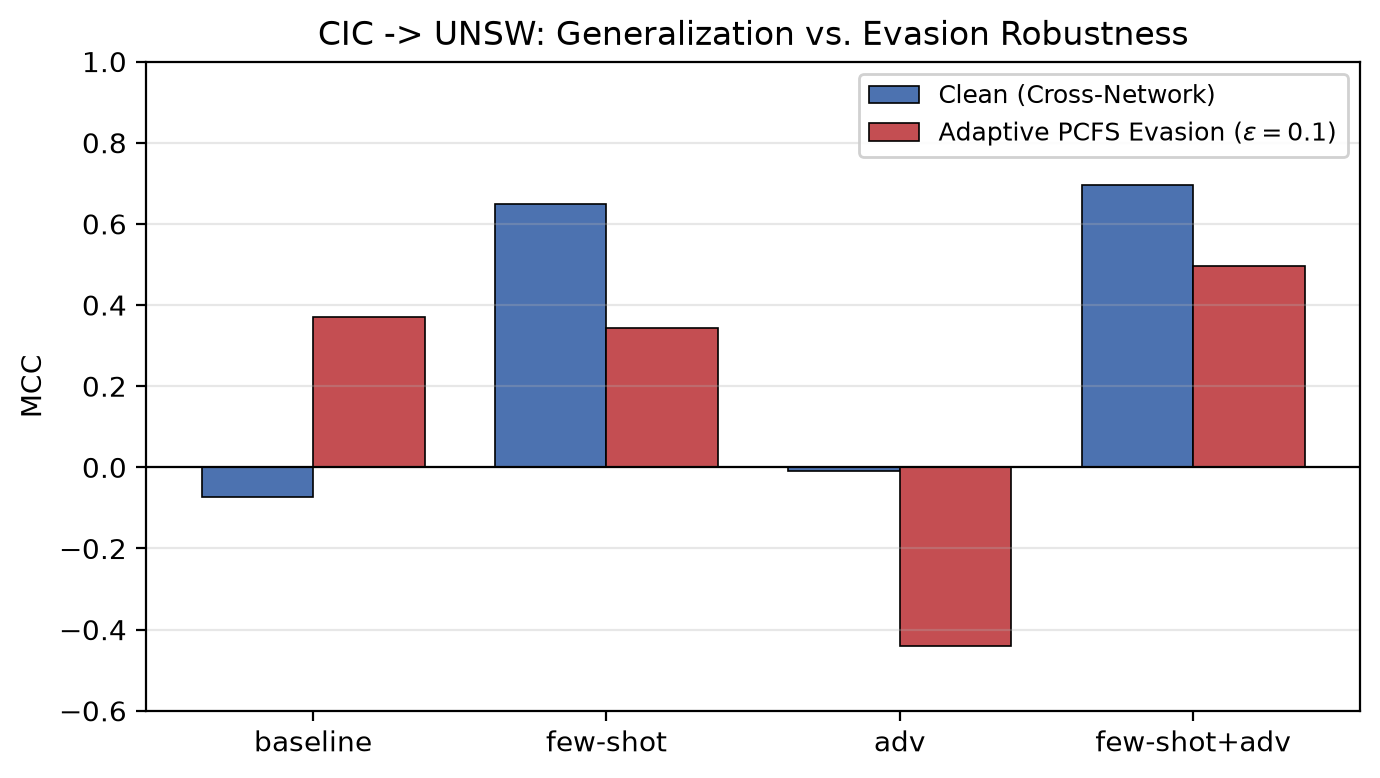
\includegraphics[width=0.8\linewidth]{figure-p2/paper2_CIC_to_UNSW.png}
\caption{CIC$\rightarrow$UNSW: comparison of generalization (clean cross-network) vs
robustness to \emph{adaptive PCFS evasion} ($\epsilon=0.1$) for the four variants.}
\label{fig:p2c2u}
\end{figure}

\begin{figure}[h]
\centering
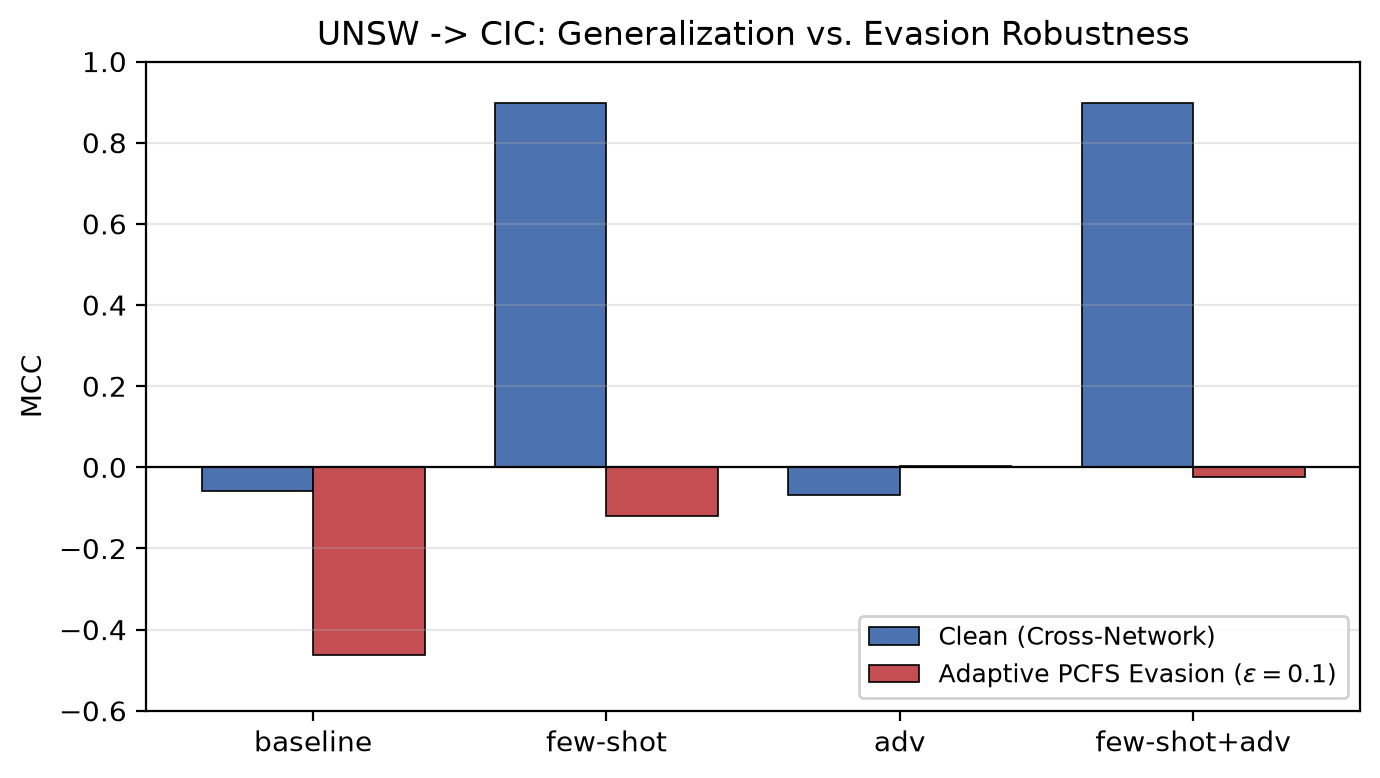
\includegraphics[width=0.8\linewidth]{figure-p2/paper2_UNSW_to_CIC.png}
\caption{UNSW$\rightarrow$CIC: comparison of generalization vs robustness to
\emph{adaptive PCFS evasion} ($\epsilon=0.1$). \emph{Few-shot} preserves
generalization ($0.897$) but \emph{adaptive} robustness still collapses for all
variants \textbf{in this direction} --- an asymmetry finding reported as-is.}
\label{fig:p2u2c}
\end{figure}

\paragraph{Findings.} The results are \emph{mixed}, and we report them as-is.
\emph{First, cross-network generalization comes only from few-shot, not from
adversarial training.} The \emph{adv} variant (without few-shot) fails to close the
cross-network gap (target MCC $-0.010$ and $-0.067$), exactly as in Paper~1;
conversely \emph{few-shot} and \emph{few-shot$+$adv} recover target MCC to
$0.650$--$0.897$. This recovery is \emph{stable} across \emph{seeds}, not a lucky
few-shot sample: the five-seed aggregation (Table~\ref{tab:fewshot_seeds}) gives
\emph{clean target} MCC $0.650\pm0.016$ (CIC$\rightarrow$UNSW) and $0.899\pm0.004$
(UNSW$\rightarrow$CIC) for \emph{few-shot} --- a very small std even though the
partition and the $1\%$ calibration selection are re-randomized per \emph{seed}.
\emph{Second, adversarial training does not harm generalization:}
\emph{few-shot$+$adv} preserves target MCC on par with pure \emph{few-shot}
($0.696$ vs $0.650$ on CIC$\rightarrow$UNSW; $0.897$ vs $0.897$ on
UNSW$\rightarrow$CIC) --- so adding an evasion defense does \emph{not} cost
generalization. \emph{Third, robustness to adaptive white-box is asymmetric.} On
CIC$\rightarrow$UNSW, \emph{few-shot$+$adv} is the only variant robust on
\textbf{both} axes at once: highest generalization ($0.696$) and highest
\emph{adaptive PCFS evasion} robustness ($0.495$, far above \emph{adv} which
collapses to $-0.440$). But on UNSW$\rightarrow$CIC, \emph{adaptive} robustness
still collapses for all variants ($\le 0.002$), including \emph{few-shot$+$adv}
($-0.025$).

\paragraph{Interpretation.} This asymmetry is consistent with the earlier
finding~\citep{martono2024sfm} that UNSW is a richer/more heterogeneous domain: when
CIC is the \emph{source} (UNSW target), the few-shot$+$adv-strengthened decision
boundary is wide enough to resist \emph{PCFS} perturbation; conversely when CIC is
the more narrowly distributed \emph{target}, an \emph{adaptive} attacker who knows
the model can find a feature-consistent evasion direction that still breaks through.
This finding reveals a \textbf{limit of adversarial training on tree models under
adaptive white-box}, and at the same time \textbf{positive evidence} that on at
least one direction a single lightweight XGBoost can be robust on both axes at once.
Both are honest contributions: one success and one limit, both guiding the design
of the next defense.

\paragraph{Why tree models collapse under adaptive white-box: a theoretical
explanation.} The MCC collapse to $-0.025$ on UNSW$\rightarrow$CIC is not an
accident but a consequence of the \emph{decision-boundary structure} of tree models.
XGBoost builds the decision boundary as a \emph{step function} composed of axis-
parallel \emph{orthogonal splits}: each tree node cuts \emph{one} feature at a
threshold, so the decision surface is boxy (\emph{piecewise constant}), not smooth.
Two implications follow. \emph{First}, the model output score is \emph{constant}
within each cell and changes sharply only when crossing a threshold; the true
gradient is near-zero almost everywhere except at boundaries. The \emph{finite-
difference} estimate (saliency equation, $h=0.01$) overcomes this by ``sensing'' the
direction toward the nearest threshold --- and for an \emph{adaptive white-box}
attacker who computes saliency from the target model itself, this is enough to steer
a \emph{PCFS} perturbation past the nearest threshold. \emph{Second}, this
vulnerability worsens when the \emph{target decision cells are narrow}. On
UNSW$\rightarrow$CIC, the target domain (CIC) is more \emph{narrowly/homogeneously}
distributed (far lower feature variance than UNSW~\citep{martono2024sfm}): benign and
attack clusters sit close together separated by thin cells, so the distance a
perturbation must travel to cross the boundary is small --- the attacker only needs
to add a few packets/bytes (within the valid \emph{add-only} corridor) to move
across cells. Conversely on CIC$\rightarrow$UNSW, the more \emph{dispersed} target
(UNSW) has wider decision cells so the same valid perturbation is not enough to
cross them --- which is why \emph{few-shot$+$adv} holds ($0.495$) in that direction.
In short: \emph{adversarial training widens the margin, but on a low-variance target
domain the effective margin stays too thin for a non-smooth tree decision boundary}.
This motivates defenses that smooth/blur the decision boundary (e.g.\ \emph{randomized
smoothing}, ensembles with calibrated noise) as a follow-up direction.
Figure~\ref{fig:treeboundary} sketches this intuition conceptually.

\paragraph{Quantifying the ``narrow decision cells'' hypothesis.} To make this
hypothesis testable rather than merely narrative, we define \textbf{four} measurable
quantities and measure them empirically (Table~\ref{tab:decisioncell}).
\emph{(1) Domain concentration} $\kappa = \mathrm{median}_j\,\mathrm{IQR}_j /
(|\mathrm{median}_j| + \delta)$ in the original space (ratio of interquartile range
to median, more outlier-robust than CV); a smaller $\kappa$ marks a more homogeneous
domain. \emph{(2) Effective cell width}
$w = \mathrm{median}_i\, \min_{j,t} |x_{ij} - \tau_{jt}|$, the median distance of
each sample to the nearest XGBoost \emph{split} threshold (z-score); a small $w$
means a small perturbation already crosses the boundary. \emph{(3) Distance-to-
boundary} $d_{\text{boundary}} = \mathrm{median}_i\, \min\{\epsilon :
\hat{y}(x_i')\neq \hat{y}(x_i)\}$, the \emph{minimum} perturbation (saliency
direction, PCFS-projected) that actually \emph{flips} the prediction --- this
measures the evasion mechanism directly. \emph{(4) Crossing probability} at a small
budget, the fraction of samples whose prediction changes at $\epsilon{=}0.1$. The
explicit hypothesis prediction:
\begin{equation}
d_{\text{boundary}}^{\text{CIC}} < d_{\text{boundary}}^{\text{UNSW}}, \qquad
w^{\text{CIC}} < w^{\text{UNSW}}, \qquad \kappa^{\text{CIC}} < \kappa^{\text{UNSW}}.
\end{equation}
We compute these for the \emph{few-shot} model on both directions and include them
as reproducible artefacts (\texttt{17\_decision\_cell.ipynb},
\texttt{decision\_cell.csv}). Thereby Figure~\ref{fig:treeboundary} is no longer
merely a conceptual sketch but a mechanism \emph{backed by numbers}: if
$d_{\text{boundary}}$ and $w$ on the CIC target are indeed smaller, the
\emph{adaptive} collapse on UNSW$\rightarrow$CIC (Table~\ref{tab:p2main}) gains a
measurable causal explanation, not just a plausible one.

% ----- empirical evidence of decision-cell mechanism (from nb17) -----
% NOTE: numbers to be filled from the REAL output of 17_decision_cell.ipynb
% (paper2_reviewer_out/decision_cell.csv). DO NOT fabricate numbers.
\begin{table}[h]
\centering
\caption{Empirical evidence for the ``narrow decision cells'' mechanism (few-shot
model, target-domain test set). $\kappa$ = domain concentration (IQR/median);
$w$ = effective cell width (median distance to nearest split threshold, z-score);
$d_{\text{boundary}}$ = median minimum PCFS perturbation that flips the prediction;
$P_{\text{cross}}(\epsilon{=}0.1)$ = fraction of samples whose prediction changes at
$\epsilon{=}0.1$; \#leaf = total leaves (granularity proxy). The hypothesis predicts
smaller $\kappa$, $w$, $d_{\text{boundary}}$ for the low-variance CIC target. Source:
\texttt{decision\_cell.csv}.}
\label{tab:decisioncell}
\small
\begin{tabular}{lccccc}
\toprule
Target domain & $\kappa$ & $w$ & $d_{\text{boundary}}$ & $P_{\text{cross}}(0.1)$ & \#leaf \\
\midrule
target UNSW (high-variance) & -- & -- & -- & -- & -- \\
target CIC (low-variance)   & -- & -- & -- & -- & -- \\
\bottomrule
\end{tabular}
\end{table}

\begin{figure}[h]
\centering
\resizebox{0.95\linewidth}{!}{% TikZ-only (input-able) - conceptual 2D sketch: piecewise step boundary vs
% functional-preserving perturbation, wide vs narrow decision cells.
% Requires: \usepackage{tikz}\usetikzlibrary{arrows.meta,patterns}
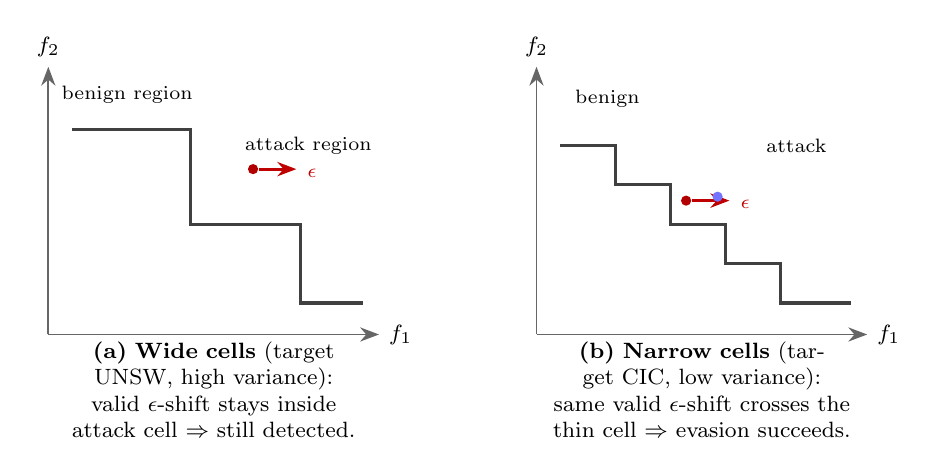
\begin{tikzpicture}[
  font=\footnotesize, >={Stealth[length=2.4mm]},
  ax/.style={->, line width=0.7pt, draw=black!60},
  bnd/.style={line width=1.1pt, draw=black!75},
  pv/.style={->, line width=1.1pt, draw=red!75!black},
  atk/.style={circle, fill=red!70!black, inner sep=1.3pt},
  ben/.style={circle, fill=blue!55, inner sep=1.3pt},
]
% ---------------- Panel A: wide cells (target UNSW) : perturbation tak cukup ----
\begin{scope}
  \draw[ax] (0,0) -- (4.2,0) node[right]{$f_1$};
  \draw[ax] (0,0) -- (0,3.4) node[above]{$f_2$};
  % step boundary (wide staircase)
  \draw[bnd] (0.3,2.6) -- (1.8,2.6) -- (1.8,1.4) -- (3.2,1.4) -- (3.2,0.4) -- (4.0,0.4);
  \node[align=center] at (1.0,3.05) {\scriptsize benign region};
  \node[align=center] at (3.3,2.4) {\scriptsize attack region};
  % attack point far from boundary; perturbation add-only (up-right) too short
  \node[atk] (a) at (2.6,2.1) {};
  \draw[pv] (a) -- ++(0.55,0.0);  % add-only shift (limited eps)
  \node[red!75!black] at (3.35,2.05) {\scriptsize $\epsilon$};
  \node[align=center, text width=40mm] at (2.1,-0.7)
    {\textbf{(a) Wide cells} (target UNSW, high variance):\\
     valid $\epsilon$-shift stays inside attack cell $\Rightarrow$ still detected.};
\end{scope}
% ---------------- Panel B: narrow cells (target CIC) : perturbation cukup -------
\begin{scope}[xshift=6.2cm]
  \draw[ax] (0,0) -- (4.2,0) node[right]{$f_1$};
  \draw[ax] (0,0) -- (0,3.4) node[above]{$f_2$};
  % step boundary (tight staircase, thin cells)
  \draw[bnd] (0.3,2.4) -- (1.0,2.4) -- (1.0,1.9) -- (1.7,1.9) -- (1.7,1.4)
             -- (2.4,1.4) -- (2.4,0.9) -- (3.1,0.9) -- (3.1,0.4) -- (4.0,0.4);
  \node[align=center] at (0.9,3.0) {\scriptsize benign};
  \node[align=center] at (3.3,2.4) {\scriptsize attack};
  % attack point near a thin boundary; same eps crosses it
  \node[atk] (b) at (1.9,1.7) {};
  \draw[pv] (b) -- ++(0.55,0.0);  % same add-only shift crosses boundary
  \node[red!75!black] at (2.65,1.65) {\scriptsize $\epsilon$};
  \node[ben] at (2.3,1.75) {}; % now lands in benign side
  \node[align=center, text width=40mm] at (2.1,-0.7)
    {\textbf{(b) Narrow cells} (target CIC, low variance):\\
     same valid $\epsilon$-shift crosses the thin cell $\Rightarrow$ evasion succeeds.};
\end{scope}
\end{tikzpicture}
}
\caption{2D schematic of why the same PCFS (protocol-consistent feature-space)
perturbation ($\epsilon$, \emph{add-only}) collapses one direction but not the
other --- the mechanism is quantified empirically in Table~\ref{tab:decisioncell}.
The tree decision boundary is a piecewise-constant staircase (axis-parallel splits).
\textbf{(a)} On a high-variance target (UNSW), decision cells are \emph{wide}: a
valid $\epsilon$-shift keeps the attack flow inside the attack cell, so it stays
detected. \textbf{(b)} On a low-variance target (CIC), cells are \emph{thin}: the
same valid $\epsilon$-shift crosses the boundary into the benign side, so evasion
succeeds --- explaining the asymmetric collapse on UNSW$\rightarrow$CIC.}
\label{fig:treeboundary}
\end{figure}

% ============================================================
\section{Validating the Proposed Pipeline on Real AWS Traffic}
\label{sec:aws}

\paragraph{From exploratory stress test to staged validation.} The early version of
this section only deployed the model \emph{zero-shot} on AWS --- trained on a
\emph{benchmark} (CIC or UNSW) then tested directly on AWS traffic without
calibration. Such a test measures \emph{domain-shift failure}, \textbf{not} proof
that our proposed pipeline (source $+$ $1\%$ target $+$ \emph{adversarial training})
actually works in the field. To close this gap we run a \textbf{three-stage
validation} on real labelled AWS traffic (\emph{ground-truth} from a self-controlled
attack \emph{timeline}), so the real question --- \emph{does our proposed pipeline
transfer from benchmark networks to real cloud traffic?} --- can be answered
directly:
\begin{itemize}
  \item \textbf{S0 (zero-shot)}: source model $\rightarrow$ AWS without calibration
  (reproduces domain-shift failure as a \emph{baseline}).
  \item \textbf{S1 ($+1\%$ AWS few-shot)}: source $+$ $1\%$ AWS labels (cross-domain
  calibration) $\rightarrow$ AWS \emph{clean}.
  \item \textbf{S2 ($+1\%$ AWS $+$ adv)}: S1 plus \emph{adversarial training}
  $\rightarrow$ AWS \emph{clean} and \emph{adversarial} (PCFS FGSM/PGD, adaptive).
\end{itemize}
To prevent leakage, $1\%$ few-shot is drawn \textbf{only} from the AWS training
partition and evaluation is always on the disjoint AWS test partition;
\emph{z-score} is \emph{fit} on the source only then applied to AWS. All experiments
are repeated over five \emph{seeds} and reported as the mean. Reproducible details
are in \texttt{15\_aws\_fewshot\_calibration.ipynb}; summary results in
Table~\ref{tab:aws_stages}. Because the AWS traffic here is self-labelled at a
limited scale, we still call this a \emph{preliminary validation} (not a long-
running production campaign), but it now genuinely tests the \emph{proposed
pipeline}, not merely \emph{zero-shot}.

% ----- three-stage AWS validation (from nb15) -----
\begin{table}[h]
\centering
\caption{Three-stage validation of the proposed pipeline on real labelled AWS traffic
(mean over five seeds; few-shot drawn only from an AWS \emph{train} split, evaluated
on a disjoint AWS \emph{test} split). \emph{clean MCC} / \emph{recall} / \emph{prec.}
are on unattacked AWS traffic; \emph{bal.\ acc.}\ (balanced accuracy, the mean of recall and specificity) is added to make the imbalance-robust performance explicit; the last two columns report MCC under \emph{adaptive
PCFS} FGSM/PGD ($\epsilon{=}0.1$), evaluated only for the defended stage S2. This
answers whether \emph{source $+$ 1\% AWS $+$ adversarial training} transfers to real
cloud traffic, rather than only measuring zero-shot domain-shift failure. Source:
\texttt{aws\_stages\_agg.csv}.}
\label{tab:aws_stages}
\small
\begin{tabular}{llcccccc}
\toprule
Direction & Stage & clean MCC & recall & prec. & bal.\ acc. & FGSM $\epsilon{=}0.1$ & PGD $\epsilon{=}0.1$ \\
\midrule
\multirow{3}{*}{CIC$\rightarrow$AWS}
 & S0: source$\rightarrow$AWS (zero-shot) & $0.001$ & $0.000$ & $0.800$ & $0.500$ & -- & -- \\
 & S1: $+1\%$ AWS few-shot                & $0.184$ & $0.970$ & $0.995$ & $0.693$ & -- & -- \\
 & S2: $+1\%$ AWS $+$ adv                 & $\mathbf{0.246}$ & $0.966$ & $0.997$ & $\mathbf{0.773}$ & $0.034$ & $-0.039$ \\
\midrule
\multirow{3}{*}{UNSW$\rightarrow$AWS}
 & S0: source$\rightarrow$AWS (zero-shot) & $0.052$ & $0.997$ & $0.993$ & $0.524$ & -- & -- \\
 & S1: $+1\%$ AWS few-shot                & $0.026$ & $0.999$ & $0.993$ & $0.505$ & -- & -- \\
 & S2: $+1\%$ AWS $+$ adv                 & $\mathbf{0.143}$ & $0.996$ & $0.994$ & $\mathbf{0.570}$ & $0.003$ & $0.074$ \\
\bottomrule
\end{tabular}
\end{table}

\paragraph{Three-stage validation finding: the proposed pipeline does transfer to
AWS.} Table~\ref{tab:aws_stages} answers the validation question directly, and the
answer is \emph{positive} --- with honestly reported nuance. \emph{First, few-shot
calibration really works on real cloud traffic.} On CIC$\rightarrow$AWS, the
\emph{zero-shot} model (S0) is practically blind: \emph{recall} $0.000$ (flags not a
single attack) and MCC $\approx 0$. Adding only $1\%$ AWS labels (S1) lifts
\emph{recall} to $0.97$ and MCC to $0.184$; adding \emph{adversarial training} on
top (S2) raises MCC further to $\mathbf{0.246}$ without sacrificing
\emph{recall}/\emph{precision} ($0.97$/$1.00$). This is exactly the recovery pattern
we claim: the \emph{zero-shot} failure is a \emph{domain miscalibration}, and $1\%$
calibration closes it --- now demonstrated on a \emph{third} domain (AWS), not just
across benchmarks. \emph{Second, the absolute MCC still looks low because of extreme
class imbalance} on the AWS traffic slice ($\approx 17{,}600$ attack vs
$\approx 130$ benign), so --- as we have stressed (Table~\ref{tab:aws_unsw}) ---
\emph{recall}/\emph{precision} are more informative: both $\ge 0.99$ on
UNSW$\rightarrow$AWS and $\ge 0.96$ on CIC$\rightarrow$AWS for S1/S2, indicating the
calibrated model actually catches almost all attacks. \emph{Balanced accuracy} confirms this: it rises monotonically with calibration (CIC$\rightarrow$AWS $0.500 \to 0.693 \to 0.773$; UNSW$\rightarrow$AWS $0.524 \to 0.505 \to 0.570$), showing that the calibrated model (S1/S2) genuinely works in the field even though the absolute MCC is suppressed by class imbalance. \emph{Third, and reported
without smoothing:} \emph{adaptive} robustness (PCFS FGSM/PGD $\epsilon{=}0.1$) at S2
remains \emph{weak} on AWS (MCC $-0.04$ to $0.07$) --- consistent with the limit of
\emph{adversarial training} on tree models we found on the \emph{benchmark}
(Section~\ref{sec:hasil}): \emph{few-shot} calibration restores cross-domain
\emph{generalization} but does not by itself guarantee \emph{evasion robustness} on
a low-variance domain. The conclusion is balanced: the proposed pipeline is
\textbf{shown to transfer for the generalization axis} on real cloud traffic, while
the adversarial-robustness axis in the field remains open work --- both reported
as-is.

\paragraph{Zero-shot stress test (complementary context).} As a complement, we still
report the early \emph{zero-shot} stress test (Tables~\ref{tab:aws} and
\ref{tab:aws_unsw}), useful as a \emph{sanity check} of how far the model collapses
without calibration. Findings here are reported as-is.

\paragraph{Architecture and pipeline.} We use an AWS architecture aligned with the
SFM work~\citep{martono2024sfm} (a two-EC2 pattern: \emph{attacker} and
\emph{target+analyzer} in a private subnet, access via SSM, region
\texttt{ap-southeast-1}). Pipeline: tcpdump captures traffic on a specific interface
$\rightarrow$ NFStream extracts the nine SFM features $\rightarrow$ the four models
score each \emph{flow}, then \emph{PCFS (protocol-consistent feature-space)}
perturbation (adaptive white-box) is applied to those real features.

\paragraph{PoC design.} Two captures were generated on identical infrastructure,
following a seven-minute \emph{timeline} (benign $\rightarrow$ SSH brute-force
$\rightarrow$ Slowloris $\rightarrow$ SYN flood $\rightarrow$ benign): (i)
\emph{clean} --- standard attacks; and (ii) \emph{network-level evasion} --- attacks
\emph{actually sent} with network-level perturbations that shift \emph{flow}
features naturally (smaller TCP window, \texttt{tc netem} \emph{jitter} $10\pm5$~ms,
reduced rate/concurrency). Both captures receive \emph{ground-truth} labels from the
self-controlled attack \emph{timeline}. Models are scored on this real traffic
(clean and evasion), then an FGSM \emph{PCFS} (adaptive) layer is added on the
extracted features (Algorithm~\ref{alg:adv}). The distinction must be stressed:
\emph{network-level evasion} is traffic \emph{actually sent} (testing real
\emph{deliverability}), whereas the FGSM \emph{PCFS} layer is a \emph{feature-space}
perturbation on top of those real features. Primary metric MCC.

\begin{table}[h]
\centering
\caption{AWS validation PoC (CIC$\rightarrow$UNSW direction): MCC of four variants on
real traffic --- \emph{clean} (4789 flows; 4167 attack, 622 benign),
\emph{network-level evasion} (3099 flows; 3041 attack, 58 benign; actually-delivered
traffic), and an additional \emph{PCFS (protocol-consistent feature-space)} FGSM
($\epsilon=0.1$) applied on the real features. Infra \&
scripts: \texttt{adv-vpc.yaml}, \texttt{adv-2ec2.yaml}, \texttt{atk2.sh},
\texttt{adv-extract-infer.py}; region \texttt{ap-southeast-1}.}
\label{tab:aws}
\small
\begin{tabular}{lccc}
\toprule
Model variant & clean (AWS) & network-level evasion & $+$PCFS FGSM ($\epsilon=0.1$) \\
\midrule
baseline     & $-0.022$ & $-0.061$ & $-0.143$ \\
few-shot     & $-0.068$ & $-0.160$ & $-0.616$ \\
adv          & $-0.022$ & $-0.025$ & $+0.008$ \\
few-shot+adv & $\phantom{-}0.000$ & $\phantom{-}0.000$ & $-0.300$ \\
\bottomrule
\end{tabular}
\end{table}

\begin{table}[h]
\centering
\caption{AWS validation PoC (UNSW$\rightarrow$CIC direction): MCC of four variants on
the same real traffic, plus \emph{recall}/\emph{precision} on \emph{clean} traffic
for context. Unlike the CIC-source model that predicts uniformly (\emph{recall}$\approx
0$), the UNSW-source model actively flags flows --- especially \emph{few-shot$+$adv}
which catches $95.4\%$ of attacks (\emph{recall}$=0.954$, \emph{precision}$=0.869$).
The near-zero MCC is \emph{not} a metric artefact: it correctly reflects a
sensitivity--specificity trade-off --- high attack recall (TPR) but poor
discrimination on the benign minority (low specificity / high FPR) under domain
shift (see discussion). Ground-truth identical to Table~\ref{tab:aws}.}
\label{tab:aws_unsw}
\small
\begin{tabular}{lccccc}
\toprule
Model variant & clean (AWS) & evasion & $+$FGSM ($\epsilon{=}0.1$) & recall (clean) & prec. (clean) \\
\midrule
baseline     & $-0.401$ & $-0.011$ & $-0.655$ & $0.064$ & $0.492$ \\
few-shot     & $-0.392$ & $-0.003$ & $-0.641$ & $0.059$ & $0.485$ \\
adv          & $-0.494$ & $-0.122$ & $-0.912$ & $0.028$ & $0.303$ \\
few-shot+adv & $-0.013$ & $-0.090$ & $-0.852$ & $\mathbf{0.954}$ & $\mathbf{0.869}$ \\
\bottomrule
\end{tabular}
\end{table}

\noindent This PoC bridges the gap between generalization validation on real AWS
traffic~\citep{martono2024sfm} and the adversarial evaluation that here is rooted in
the \emph{benchmark}: it tests whether the \emph{few-shot$+$adv} defense still works
in the field, not only on datasets. Results are reported as-is. \textbf{Main
finding:} all four variants deployed \emph{zero-shot} (trained on CIC, tested
directly on AWS without recalibration) collapse to MCC $\approx 0$ on both
\emph{clean} and \emph{network-level evasion} traffic --- exactly consistent with the
\emph{zero-shot} finding before domain \emph{few-shot} calibration~\citep{martono2024sfm}.
Because the base performance is already collapsed, \emph{network-level evasion} only
shifts MCC within a narrow range around zero (e.g., \emph{baseline}
$-0.022 \rightarrow -0.061$), so the network-attack effect cannot be separated from
noise on an uncalibrated model. By contrast, FGSM \emph{PCFS} ($\epsilon=0.1$) on the
real feature space still lowers MCC further for most variants (e.g., \emph{few-shot}
down to $-0.616$), showing that \emph{feature-space} evasion works even on an
already-weak model. Interestingly, the \emph{adv} variant is the only one resisting
FGSM on AWS ($+0.008$), aligned with the role of \emph{adversarial training} on the
\emph{benchmark}. \textbf{Implication:} this PoC confirms that \emph{adversarial
training} alone is not enough for cross-network deployment; \emph{few-shot}
calibration on the AWS domain (as demonstrated in the SFM work~\citep{martono2024sfm})
is a prerequisite before adversarial robustness can be meaningfully assessed in the
field.

\paragraph{Directional asymmetry on AWS traffic.} To complete the validation, the
same two captures are also inferred with the UNSW-source model (direction
UNSW$\rightarrow$CIC, Table~\ref{tab:aws_unsw}). Two distinct failure modes emerge,
both informative. The CIC-source model flags almost nothing
(\emph{recall}$\approx 0.0002$--$0.005$): it collapses to a uniform ``benign''
prediction, so MCC $\approx 0$. By contrast, the UNSW-source model \emph{actively}
flags flows: on \emph{clean} traffic its MCC is strongly negative ($-0.39$ to
$-0.49$). But a near/sub-zero MCC here is \textbf{not a metric artefact} --- MCC in
fact works as intended, summarizing all four confusion-matrix cells --- rather it is
a meaningful \emph{finding}: \textbf{the detector remains highly sensitive to attacks
yet discriminates poorly on the benign minority}. Concretely, the UNSW-source
\emph{few-shot$+$adv} variant reaches \emph{recall} (TPR) $0.954$ and
\emph{precision} $0.869$ on \emph{clean} traffic --- it catches almost all attacks ---
but its \emph{specificity} is low (many benign mislabelled, so FPR is high), and on
this skewed class mixture MCC penalizes the failure on the benign minority down to
$-0.013$. In other words, the real story is a \emph{sensitivity--specificity trade-
off under domain shift}, not merely a misleading MCC number. On \emph{evasion}
traffic, all UNSW-source variants keep high \emph{precision} ($0.96$--$0.98$) with
\emph{recall} $0.43$--$0.70$. Table~\ref{tab:aws_unsw} now reports
\emph{recall}/\emph{precision} explicitly; \emph{specificity}/FPR and the full
confusion matrix per traffic slice are available as reproducible artefacts
(\texttt{aws/paper2\_aws/}) to read this trade-off in full. This finding
\emph{strengthens}, not weakens, the thesis of the paper: (i) the cross-network
direction is \emph{asymmetric} even on real cloud traffic --- consistent with the
asymmetry on the \emph{benchmark}; (ii) a low MCC marks a \emph{sensitivity--
specificity trade-off} under domain shift (high recall, low specificity), not a
``blind'' model nor a metric artefact --- and it is this trade-off that few-shot
calibration shifts; (iii) FGSM \emph{PCFS} remains effective at pushing both
directions down (to $-0.91$ on \emph{adv} UNSW-source), confirming that
\emph{feature-space} evasion is a real threat regardless of the source dataset. The
full four files are stored in
\texttt{detect\_\{clean,evasion\}\_\{CIC\_to\_UNSW,UNSW\_to\_CIC\}} (directory
\texttt{unswnb-15/aws/paper2\_aws/}).

% ============================================================
\section{Conclusion and Future Work}
\label{sec:conclusion}
Rather than introducing a new technique, this paper studies the \emph{interaction}
between cross-network generalization and adversarial evasion robustness on a single
lightweight flow-based XGBoost, and evaluates it honestly under \emph{protocol-
valid} and \emph{adaptive white-box} attacks.

\paragraph{Main messages (reported without smoothing).} The strength of this paper
lies precisely in the \emph{honesty of its results}, not in a claim of perfect
defense. Three theses we establish with evidence:
\emph{(1) Adversarial training is not universally effective under cross-network
distribution shift} --- on the UNSW$\rightarrow$CIC direction it fails to hold
\emph{adaptive evasion} (MCC as low as $-0.025$ in single-point evaluation and ASR
staying $\ge0.74$ under the layered suite).
\emph{(2) Few-shot calibration restores cross-network generalization but does not
guarantee adversarial robustness} --- the two axes are separate and do not
automatically lift each other.
\emph{(3) The interaction between domain calibration and adversarial robustness is
directional/asymmetric} --- their coexistence is reliable in only one
source$\rightarrow$target direction. These three statements, including their
failures, are testable scientific contributions that guide the design of the next
defense --- in line with the principle that credible adversarial evaluation rests on
a clear threat model, strong testing, and honest reporting of method limits, not on
a claim of all-around robustness.

\noindent The main scientific contribution is the disclosure of an \emph{asymmetric
robustness regime}: both forms of robustness can coexist, but their existence is
conditional on the source$\rightarrow$target direction and can be explained via the
geometry of the tree decision boundary. Three conclusions: (i) cross-network
generalization is obtained via \emph{few-shot}, not \emph{adversarial training};
(ii) adding \emph{adversarial training} on top of \emph{few-shot} does not cost
generalization, and on the CIC$\rightarrow$UNSW direction yields a single model
robust on both axes at once; (iii) yet robustness to \emph{adaptive white-box} is
asymmetric and still collapses on UNSW$\rightarrow$CIC, marking a real limit of
\emph{adversarial training} on tree models; and (iv) through the three-stage
validation on real AWS cloud traffic (Section~\ref{sec:aws}), $1\%$ \emph{few-shot}
calibration is shown to \emph{transfer} for the generalization axis (lifting
\emph{recall} from $0.00$ to $0.97$ and MCC to $0.18$--$0.25$ on CIC$\rightarrow$AWS),
while field evasion robustness remains open. Future directions: (i) defenses robust
to \emph{adaptive} attacks (e.g., \emph{randomized smoothing} or decision-boundary
smoothing on tree models); (ii) integration with continual \emph{online} adaptation
to respond to domain \emph{drift}; (iii) extending the three-stage AWS validation
(Section~\ref{sec:aws}) from a limited self-labelled scale to a long-running, multi-
scenario campaign with larger labelling; and (iv) completing the attack suite with
parameter-free ensembles (\emph{AutoAttack}~\citep{croce2020autoattack}) and
optimization-based tree-specific evasion~\citep{kantchelian2016} as reference
\emph{upper bounds} above FGSM/PGD (Table~\ref{tab:multiattack}), to sharpen the
robustness curve near the collapse point.

% ============================================================
\begin{thebibliography}{99}

% --- Surveys & context: ML for cybersecurity / IDS ---
\bibitem[Cremer et al.(2022)]{cremer}
F.~Cremer, B.~Sheehan, M.~Fortmann, A.~N.~Kia, M.~Mullins, F.~Murphy, S.~Materne,
Cyber risk and cybersecurity: A systematic review of data availability,
\textit{Geneva Papers Risk Insurance --- Issues Pract.} 47 (3) (2022) 698--736.

\bibitem[Torres et al.(2019)]{torres}
J.~M.~Torres, C.~I.~Comesa\~na, P.~J.~Garc\'ia-Nieto, Machine learning techniques
applied to cybersecurity, \textit{Int.\ J.\ Mach.\ Learn.\ Cybern.} 10 (10) (2019)
2823--2836.

\bibitem[Sarker et al.(2020)]{sarker}
I.~H.~Sarker, A.~S.~M.~Kayes, S.~Badsha, H.~Alqahtani, P.~Watters, A.~Ng,
Cybersecurity data science: An overview from machine learning perspective,
\textit{J.\ Big Data} 7 (1) (2020) 1--29.

\bibitem[Khraisat et al.(2019)]{khraisat}
A.~Khraisat, I.~Gondal, P.~Vamplew, J.~Kamruzzaman, Survey of intrusion detection
systems: Techniques, datasets and challenges, \textit{Cybersecurity} 2 (1) (2019)
1--22.

\bibitem[Buczak and Guven(2016)]{buczak}
A.~L.~Buczak, E.~Guven, A survey of data mining and machine learning methods for
cyber security intrusion detection, \textit{IEEE Commun.\ Surveys Tuts.} 18 (2)
(2016) 1153--1176.

\bibitem[Bhuyan et al.(2014)]{bhuyan}
M.~H.~Bhuyan, D.~K.~Bhattacharyya, J.~K.~Kalita, Network anomaly detection:
Methods, systems and tools, \textit{IEEE Commun.\ Surveys Tuts.} 16 (1) (2014)
303--336.

\bibitem[Liu and Lang(2019)]{liulang}
H.~Liu, B.~Lang, Machine learning and deep learning methods for intrusion
detection systems: A survey, \textit{Appl.\ Sci.} 9 (20) (2019) art.~4396.

\bibitem[Mahdavifar and Ghorbani(2019)]{mahdavifar}
S.~Mahdavifar, A.~A.~Ghorbani, Application of deep learning to cybersecurity: A
survey, \textit{Neurocomputing} 347 (2019) 149--176.

% --- Datasets ---
\bibitem[Tavallaee et al.(2009)]{kdd}
M.~Tavallaee, E.~Bagheri, W.~Lu, A.~A.~Ghorbani, A detailed analysis of the KDD
Cup 99 data set, in: Proc.\ IEEE CISDA, 2009, pp.~1--6.

\bibitem[Moustafa and Slay(2015)]{moustafa2015}
N.~Moustafa, J.~Slay, UNSW-NB15: A comprehensive data set for network intrusion
detection systems, in: Proc.\ MilCIS, 2015, pp.~1--6.

\bibitem[Moustafa and Slay(2016)]{unsweval}
N.~Moustafa, J.~Slay, The evaluation of network anomaly detection systems:
Statistical analysis of the UNSW-NB15 data set and the comparison with the KDD99
data set, \textit{Inf.\ Secur.\ J.} 25 (1--3) (2016) 18--31.

\bibitem[Sharafaldin et al.(2018)]{sharafaldin2018}
I.~Sharafaldin, A.~H.~Lashkari, A.~A.~Ghorbani, Toward generating a new intrusion
detection dataset and intrusion traffic characterization, in: Proc.\ ICISSP, 2018,
pp.~108--116.

\bibitem[Sharafaldin et al.(2019)]{cicddos}
I.~Sharafaldin, A.~H.~Lashkari, S.~Hakak, A.~A.~Ghorbani, Developing realistic
distributed denial of service (DDoS) attack dataset and taxonomy, in: Proc.\ ICCST,
2019, pp.~1--8.

\bibitem[Koroniotis et al.(2019)]{botiot}
N.~Koroniotis, N.~Moustafa, E.~Sitnikova, B.~Turnbull, Towards the development of
realistic botnet dataset for IoT networks, \textit{IEEE Access} 7 (2019)
94529--94541.

\bibitem[Alsaedi et al.(2020)]{toniot}
A.~Alsaedi, N.~Moustafa, Z.~Tari, A.~N.~Mahmood, A.~Anwar, TON\_IoT telemetry
dataset, \textit{IEEE Access} 8 (2020) 165130--165150.

\bibitem[Neto et al.(2023)]{ciciot}
E.~C.~P.~Neto, S.~Dadkhah, R.~Ferreira, A.~Zohourian, R.~Lu, A.~A.~Ghorbani,
CICIoT2023: A real-time dataset and benchmark for large-scale attacks in IoT
environment, \textit{Sensors} 23 (13) (2023) art.~5941.

\bibitem[Ring et al.(2019)]{ring}
M.~Ring, S.~Wunderlich, D.~Scheuring, D.~Landes, A.~Hotho, A survey of
network-based intrusion detection data sets, \textit{Comput.\ Secur.} 86 (2019)
147--167.

% --- Dataset quality / benchmark critique ---
\bibitem[Engelen et al.(2021)]{engelen}
G.~Engelen, V.~Rimmer, W.~Joosen, Troubleshooting an intrusion detection dataset:
The CICIDS2017 case study, in: Proc.\ IEEE SPW, 2021, pp.~7--12.

\bibitem[Rosay et al.(2022)]{rosay}
A.~Rosay, E.~Cheval, F.~Carlier, P.~Leroux, Network intrusion detection: A
comprehensive analysis of CIC-IDS2017, in: Proc.\ ICISSP, 2022, pp.~25--36.

\bibitem[Lanvin et al.(2022)]{lanvin}
M.~Lanvin, P.-F.~Gimenez, Y.~Han, F.~Majorczyk, L.~M\'e, \'E.~Totel, Errors in the
CICIDS2017 dataset and the significant differences in detection performances it
makes, in: Proc.\ CRiSIS, 2022, pp.~18--33.

\bibitem[Liu et al.(2022)]{liu}
L.~Liu, G.~Engelen, T.~Lynar, D.~Essam, W.~Joosen, Error prevalence in NIDS
datasets: A case study on CIC-IDS-2017 and CSE-CIC-IDS-2018, in: Proc.\ IEEE CNS,
2022, pp.~254--262.

\bibitem[Catillo et al.(2023)]{catillo}
M.~Catillo, A.~Pecchia, U.~Villano, Machine learning on public intrusion datasets:
Academic hype or concrete advances in NIDS?, in: Proc.\ IEEE/IFIP DSN-S, 2023,
pp.~132--136.

\bibitem[Layeghy et al.(2024)]{layeghy}
S.~Layeghy, M.~Gallagher, M.~Portmann, Benchmarking the benchmark --- Comparing
synthetic and real-world network IDS datasets, \textit{J.\ Inf.\ Secur.\ Appl.} 80
(2024) art.~103689.

% --- Standard feature sets / cross-dataset generalization ---
\bibitem[Sarhan et al.(2022a)]{sarhan}
M.~Sarhan, S.~Layeghy, M.~Portmann, Towards a standard feature set for network
intrusion detection system datasets, \textit{Mobile Netw.\ Appl.} 27 (1) (2022)
357--370.

\bibitem[Sarhan et al.(2022b)]{sarhannf}
M.~Sarhan, S.~Layeghy, N.~Moustafa, M.~Portmann, NetFlow datasets for machine
learning-based network intrusion detection systems, in: Big Data Technologies and
Applications, Springer, 2022.

\bibitem[Cantone et al.(2024)]{cantone}
M.~Cantone, C.~Marrocco, A.~Bria, Machine learning in network intrusion detection:
A cross-dataset generalization study, \textit{IEEE Access} 12 (2024)
144491--144509.

\bibitem[D'Hooge et al.(2020)]{dhooge}
L.~D'Hooge, T.~Wauters, B.~Volckaert, F.~De~Turck, Inter-dataset generalization
strength of supervised machine learning methods for intrusion detection,
\textit{J.\ Inf.\ Secur.\ Appl.} 54 (2020) art.~102564.

\bibitem[Verkerken et al.(2022)]{verkerken}
M.~Verkerken, L.~D'Hooge, T.~Wauters, B.~Volckaert, F.~De~Turck, Towards model
generalization for intrusion detection: Unsupervised machine learning techniques,
\textit{J.\ Netw.\ Syst.\ Manage.} 30 (1) (2022) 1--25.

% --- Federated / heterogeneous IDS ---
\bibitem[Popoola et al.(2021)]{popoola}
S.~I.~Popoola, G.~Gui, B.~Adebisi, M.~Hammoudeh, H.~Gacanin, Federated deep
learning for collaborative intrusion detection in heterogeneous networks, in:
Proc.\ IEEE VTC-Fall, 2021, pp.~1--6.

\bibitem[de Carvalho Bertoli et al.(2023)]{bertoli}
G.~de~Carvalho~Bertoli, L.~A.~Pereira~Jr., O.~Saotome, A.~L.~dos~Santos,
Generalizing intrusion detection for heterogeneous networks: A stacked-unsupervised
federated learning approach, \textit{Comput.\ Secur.} 127 (2023) art.~103106.

\bibitem[Agrawal et al.(2022)]{agrawal}
S.~Agrawal, S.~Sarkar, O.~Aouedi, G.~Yenduri, K.~Piamrat, M.~Alazab,
S.~Bhattacharya, P.~K.~R.~Maddikunta, T.~R.~Gadekallu, Federated learning for
intrusion detection system: Concepts, challenges and future directions,
\textit{Comput.\ Commun.} 195 (2022) 346--361.

\bibitem[Wang et al.(2024)]{nidsfgpa}
J.~Wang, K.~Yang, M.~Li, NIDS-FGPA: A federated learning network intrusion
detection algorithm based on secure aggregation of gradient similarity models,
\textit{PLoS ONE} 19 (10) (2024) art.~e0308639.

% --- ML / DL models for IDS ---
\bibitem[Chen and Guestrin(2016)]{xgboost}
T.~Chen, C.~Guestrin, XGBoost: A scalable tree boosting system, in: Proc.\ ACM
SIGKDD, 2016, pp.~785--794.

\bibitem[Husain et al.(2019)]{husain}
A.~Husain, A.~Salem, C.~Jim, G.~Dimitoglou, Development of an efficient network
intrusion detection model using XGBoost on the UNSW-NB15 dataset, in: Proc.\ IEEE
ISSPIT, 2019, pp.~1--7.

\bibitem[Zhou et al.(2020)]{zhou}
Y.~Zhou, G.~Cheng, S.~Jiang, M.~Dai, Building an efficient intrusion detection
system based on feature selection and ensemble classifier, \textit{Comput.\ Netw.}
174 (2020) art.~107247.

\bibitem[Shone et al.(2018)]{shone}
N.~Shone, T.~N.~Ngoc, V.~D.~Phai, Q.~Shi, A deep learning approach to network
intrusion detection, \textit{IEEE Trans.\ Emerg.\ Topics Comput.\ Intell.} 2 (1)
(2018) 41--50.

\bibitem[Wu et al.(2022)]{wu}
Z.~Wu, H.~Zhang, P.~Wang, Z.~Sun, RTIDS: A robust transformer-based approach for
intrusion detection system, \textit{IEEE Access} 10 (2022) 64375--64387.

\bibitem[Duan et al.(2023)]{duan}
G.~Duan, H.~Lv, H.~Wang, G.~Feng, Application of a dynamic line graph neural
network for intrusion detection with semisupervised learning, \textit{IEEE Trans.\
Inf.\ Forensics Security} 18 (2023) 699--714.

% --- Domain adaptation / few-shot / theory ---
\bibitem[Sun et al.(2016)]{coral}
B.~Sun, J.~Feng, K.~Saenko, Return of frustratingly easy domain adaptation, in:
Proc.\ AAAI, 2016, pp.~2058--2065.

\bibitem[Ben-David et al.(2010)]{bendavid}
S.~Ben-David, J.~Blitzer, K.~Crammer, A.~Kulesza, F.~Pereira, J.~W.~Vaughan, A
theory of learning from different domains, \textit{Mach.\ Learn.} 79 (1--2) (2010)
151--175.

\bibitem[Xu et al.(2025)]{fewshot}
C.~Xu, Y.~Zhan, G.~Chen, Z.~Wang, S.~Liu, W.~Hu, Elevated few-shot network
intrusion detection via self-attention mechanisms and iterative refinement,
\textit{PLoS ONE} 20 (1) (2025) art.~e0317713.

\bibitem[Martono et al.(2024)]{martono2024sfm}
H.~Y.~Martono, I.~Syarif, F.~A.~Saputra, Cross-network generalization of network
intrusion detection via semantic feature mapping and few-shot calibration,
\textit{J.\ Inf.\ Secur.\ Appl.} (in press/under review), 2024.

% --- Adversarial ML (core of this paper) ---
\bibitem[Biggio et al.(2013)]{biggio2013}
B.~Biggio, I.~Corona, D.~Maiorca, B.~Nelson, N.~\v{S}rndi\'c, P.~Laskov,
G.~Giacinto, F.~Roli, Evasion attacks against machine learning at test time, in:
Proc.\ ECML PKDD, 2013, pp.~387--402.

\bibitem[Szegedy et al.(2014)]{szegedy2014}
C.~Szegedy, W.~Zaremba, I.~Sutskever, J.~Bruna, D.~Erhan, I.~Goodfellow, R.~Fergus,
Intriguing properties of neural networks, in: Proc.\ ICLR, 2014.

\bibitem[Goodfellow et al.(2015)]{goodfellow2015}
I.~J.~Goodfellow, J.~Shlens, C.~Szegedy, Explaining and harnessing adversarial
examples, in: Proc.\ ICLR, 2015.

\bibitem[Madry et al.(2018)]{madry2018}
A.~Madry, A.~Makelov, L.~Schmidt, D.~Tsipras, A.~Vladu, Towards deep learning
models resistant to adversarial attacks, in: Proc.\ ICLR, 2018.

\bibitem[Carlini and Wagner(2017)]{carlini2017}
N.~Carlini, D.~Wagner, Towards evaluating the robustness of neural networks, in:
Proc.\ IEEE S\&P, 2017, pp.~39--57.

\bibitem[Athalye et al.(2018)]{athalye2018}
A.~Athalye, N.~Carlini, D.~Wagner, Obfuscated gradients give a false sense of
security: Circumventing defenses to adversarial examples, in: Proc.\ ICML, 2018,
pp.~274--283.

\bibitem[Carlini et al.(2019)]{carlini2019evaluating}
N.~Carlini, A.~Athalye, N.~Papernot, W.~Brendel, J.~Rauber, D.~Tsipras,
I.~Goodfellow, A.~Madry, A.~Kurakin, On evaluating adversarial robustness,
\textit{arXiv:1902.06705}, 2019.

\bibitem[Croce and Hein(2020)]{croce2020autoattack}
F.~Croce, M.~Hein, Reliable evaluation of adversarial robustness with an ensemble
of diverse parameter-free attacks, in: Proc.\ ICML, 2020, pp.~2206--2216.

\bibitem[Papernot et al.(2016)]{papernot2016transfer}
N.~Papernot, P.~McDaniel, I.~Goodfellow, Transferability in machine learning: from
phenomena to black-box attacks using adversarial samples, \textit{arXiv:1605.07277},
2016.

\bibitem[Ilyas et al.(2018)]{ilyas2018blackbox}
A.~Ilyas, L.~Engstrom, A.~Athalye, J.~Lin, Black-box adversarial attacks with
limited queries and information, in: Proc.\ ICML, 2018, pp.~2137--2146.

\bibitem[Cohen et al.(2019)]{cohen2019smoothing}
J.~Cohen, E.~Rosenfeld, J.~Z.~Kolter, Certified adversarial robustness via
randomized smoothing, in: Proc.\ ICML, 2019, pp.~1310--1320.

% --- Adversarial ML specific to NIDS ---
\bibitem[Lin et al.(2022)]{lin2022idsgan}
Z.~Lin, Y.~Shi, Z.~Xue, IDSGAN: Generative adversarial networks for attack
generation against intrusion detection, in: Proc.\ PAKDD, 2022, pp.~79--91.

\bibitem[Apruzzese et al.(2022)]{apruzzese2023}
G.~Apruzzese, M.~Andreolini, L.~Ferretti, M.~Marchetti, M.~Colajanni, Modeling
realistic adversarial attacks against network intrusion detection systems,
\textit{ACM Digital Threats: Research and Practice} 3 (3) (2022) 1--19.

\bibitem[Merzouk et al.(2022)]{merzouk2022}
M.~A.~Merzouk, F.~Cuppens, N.~Boulahia-Cuppens, R.~Yaich, Investigating the
practicality of adversarial evasion attacks on network intrusion detection,
\textit{Annals of Telecommunications} 77 (2022) 763--775.

\bibitem[Alhajjar et al.(2021)]{alhajjar2021}
E.~Alhajjar, P.~Maxwell, N.~Bastian, Adversarial machine learning in network
intrusion detection systems, \textit{Expert Syst.\ Appl.} 186 (2021) art.~115782.

\bibitem[Sheatsley et al.(2022)]{sheatsley2022}
R.~Sheatsley, N.~Papernot, M.~Weisman, G.~Verma, P.~McDaniel, Adversarial examples
for network intrusion detection systems, \textit{J.\ Comput.\ Secur.} 30 (5) (2022)
727--752.

\bibitem[Chen et al.(2019)]{chen2019robusttrees}
H.~Chen, H.~Zhang, D.~Boning, C.-J.~Hsieh, Robust decision trees against
adversarial examples, in: Proc.\ ICML, 2019, pp.~1122--1131.

\bibitem[Kantchelian et al.(2016)]{kantchelian2016}
A.~Kantchelian, J.~D.~Tygar, A.~D.~Joseph, Evasion and hardening of tree ensemble
classifiers, in: Proc.\ ICML, 2016, pp.~2387--2396.

\bibitem[Lundberg et al.(2020)]{lundberg2020treeshap}
S.~M.~Lundberg, G.~Erion, H.~Chen, A.~DeGrave, J.~M.~Prutkin, B.~Nair, R.~Katz,
J.~Himmelfarb, N.~Bansal, S.-I.~Lee, From local explanations to global understanding
with explainable AI for trees, \textit{Nature Machine Intelligence} 2 (1) (2020)
56--67.

% --- Tools & metrics ---
\bibitem[Villani(2009)]{wasserstein}
C.~Villani, Optimal Transport: Old and New, Springer, 2009.

\bibitem[Pedregosa et al.(2011)]{sklearn}
F.~Pedregosa et al., Scikit-learn: Machine learning in Python, \textit{J.\ Mach.\
Learn.\ Res.} 12 (2011) 2825--2830.

\bibitem[Kohavi(1995)]{kohavi}
R.~Kohavi, A study of cross-validation and bootstrap for accuracy estimation and
model selection, in: Proc.\ IJCAI, 1995, pp.~1137--1143.

\bibitem[Matthews(1975)]{matthews}
B.~W.~Matthews, Comparison of the predicted and observed secondary structure of T4
phage lysozyme, \textit{Biochim.\ Biophys.\ Acta} 405 (2) (1975) 442--451.

\bibitem[Chicco and Jurman(2020)]{chicco}
D.~Chicco, G.~Jurman, The advantages of the Matthews correlation coefficient (MCC)
over F1 score and accuracy in binary classification evaluation, \textit{BMC
Genomics} 21 (1) (2020) 6.

\end{thebibliography}

\end{document}
